\chapter{Real Data}
Finally, we also performed inference on a real FMRI scan. The scanner we used...
%... more specifics...

Before performing tests on a full image, I tested the results of the particle filter
on regions deemed active and non-active by statistical parametric mapping. 
This served the purpose of tuning the priors to reasonable levels etc.
After that, the particle filter was applied to every voxel in an FMRI 
image individualy, and the results were put into a parameter map 
image. Additionally, the resulting MSE and square-root MSE were placed
into images for further analysis.

\section{Single-Voxel Analysis}
This section discusses the results when the particle filter was
applied on a single voxel. The parameters are the same as
those used later for entire image analysis; however, the results
are more in-depth. 

The run-time for a single voxel depends on the several factors. First, the
overall length of the signal being analyzed. For 1000 measurements it takes
about 10 to 15 minutes. On the other hand, in real circumstances the
length is only around 150 measurements. The number of  integration
can certainly make a large difference, however dropping below 1000 (.001 seconds)
is definitely not recommended. 

For a period I considered 1000 to be a
fine number; however when generating simulated data I found that every once
in a while 1000 was not enough. This is problematic in the actual particle
filter since, given the large number of simultaneous integrations taking 
place, its likely that a few particles will fail and be weighted at 0 because
of this problem. Additionally, because the typical case where a failure would
occur is at fast moving times/parameters the particles all tend to fail together.
The result is particle deprivation - no particles with non-zero weights remain.
The other possible outcome is that low time constant particles get pruned resulting
in excessively smoothed estimates for the time series'. Its possible that a
kind of stop-gap measure could be put into place; wherein particles that are
about to be set to NaN are integrated again with finer grained steps. However
many times the non-real results don't occur until several time steps after the 
numbers get strange. So for instance, the timestep was too long, allowing 
$f$ to go negative, resulting in extremely large values of $q$. There are many
different ways where this sort of event can occur, and unfortunately sometimes
there is no way to get back to before the state starting going out of control.

Another crucial factor for run time is how long before the first re-sampling 
occurs. Because the prior is represented initially with significantly more
particles, if the model fits very well, or for some reason the effective
number of particles stays high, resampling could take a long time to occur.
When this happens the particles filter can take a factor of 10 longer to run.
However, if the particle count isn't initially set high, there is a much larger
chance of particle deprivation occurring. Since there is no real way to know
how long it will take to resmaple the first time, there is little the 
algorithm can do to fix this (except perhaps forcing resampling after
some period of time). On the other end of the spectrum, if the time
series doesn't match the model at all, particle deprivation will occur extremely
quickly.  The upshot of this is that the particle filter is able to 
identify these sections very quickly, and thus not waste much time there.
The difficulty though, is the regions in between the perfect fit and the
awful fit. If particle deprivation does occur, did it occur randomly to an
activated region or did it occur inevitably because the region doesn't fit.
The reason for having so many initial particles is to give density to the
distribution to make false negatives more rare. Perhaps the correct method
is to still set the initial particles very high, but if for a long time no
resampling occurs, halve the standard deviation of the measurement error.
Thus, if the weighting function is not discriminating enough, force it 
to be more picky about the results. Of course this could lead to particle
deprivation as well if the standard deviation is brought down too quickly.
Of course, if a fat-tailed distribution is used for the weighting function,
or the standard deviation of a Gaussian weighting function is sufficiently large,
the particle filter will simply converge to meaningless values. The question
of whether 

\begin{figure}
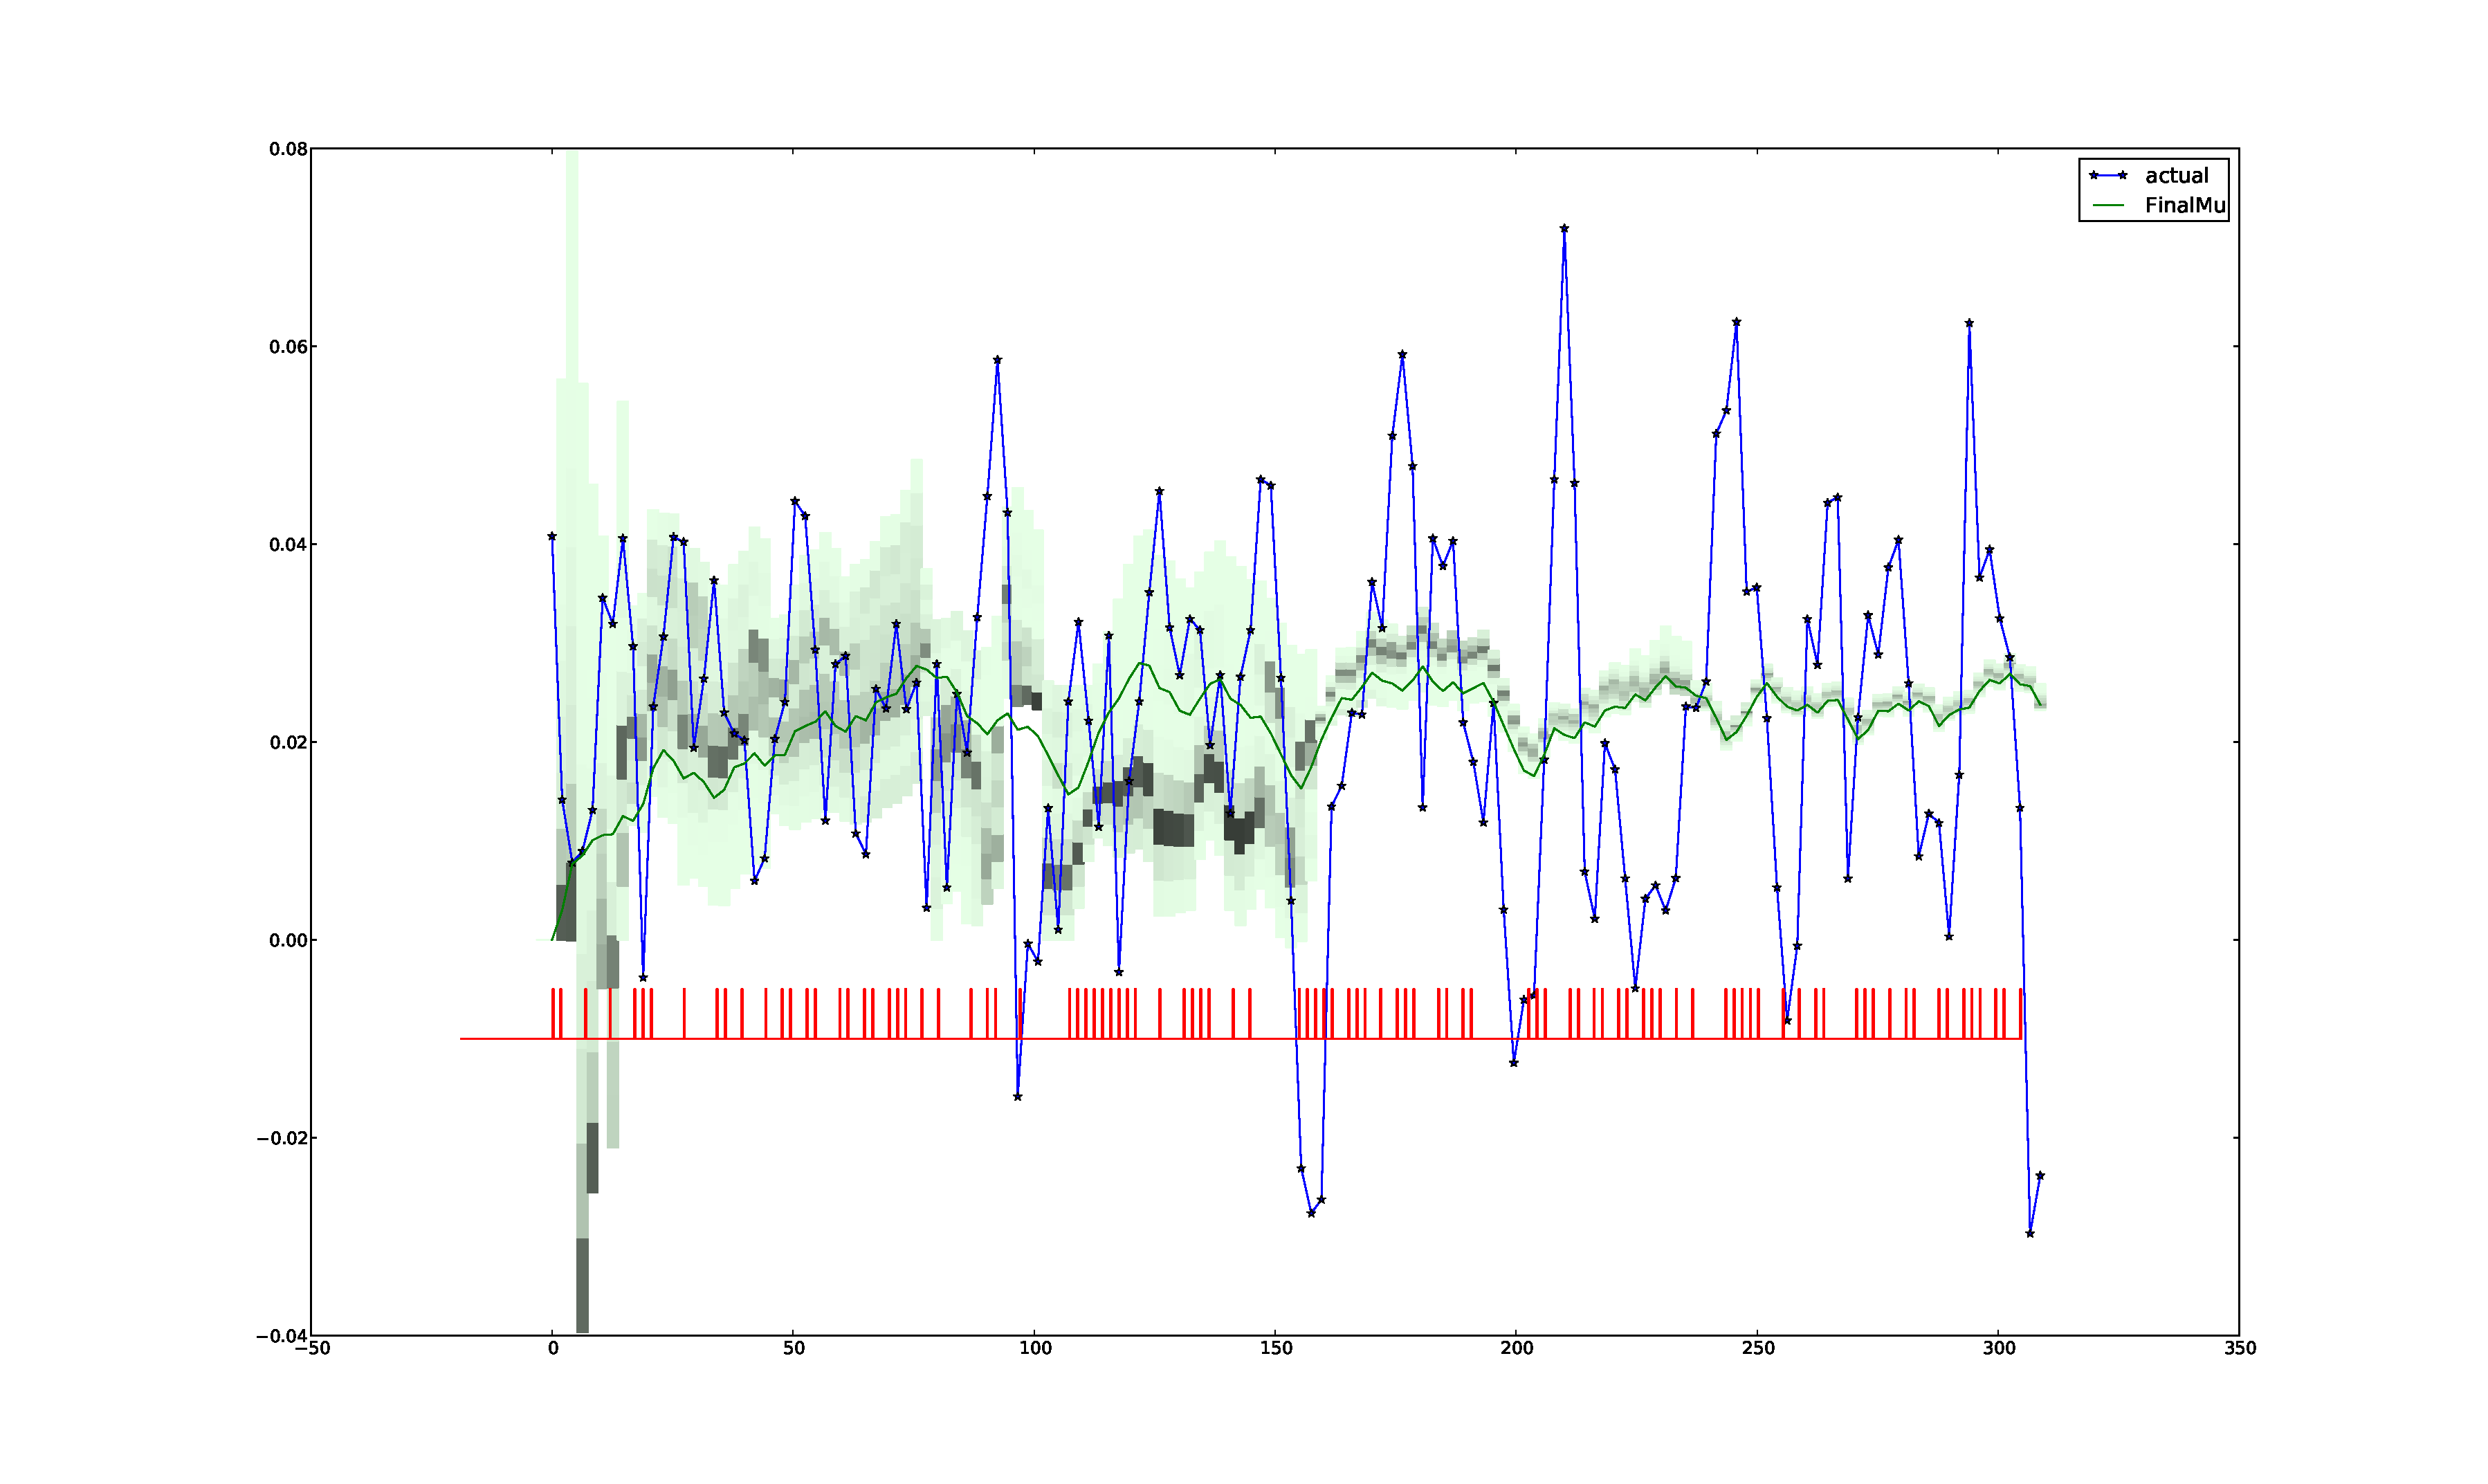
\includegraphics[clip=true,trim=10cm 4cm 10cm 4cm, width=16cm]{images/inactive_illogical}
\caption{Particle Filter converging to values that make little sense,
because the voxel did not correlate with the input in any known way}
\label{fig:badfit}
\end{figure}

\begin{figure}
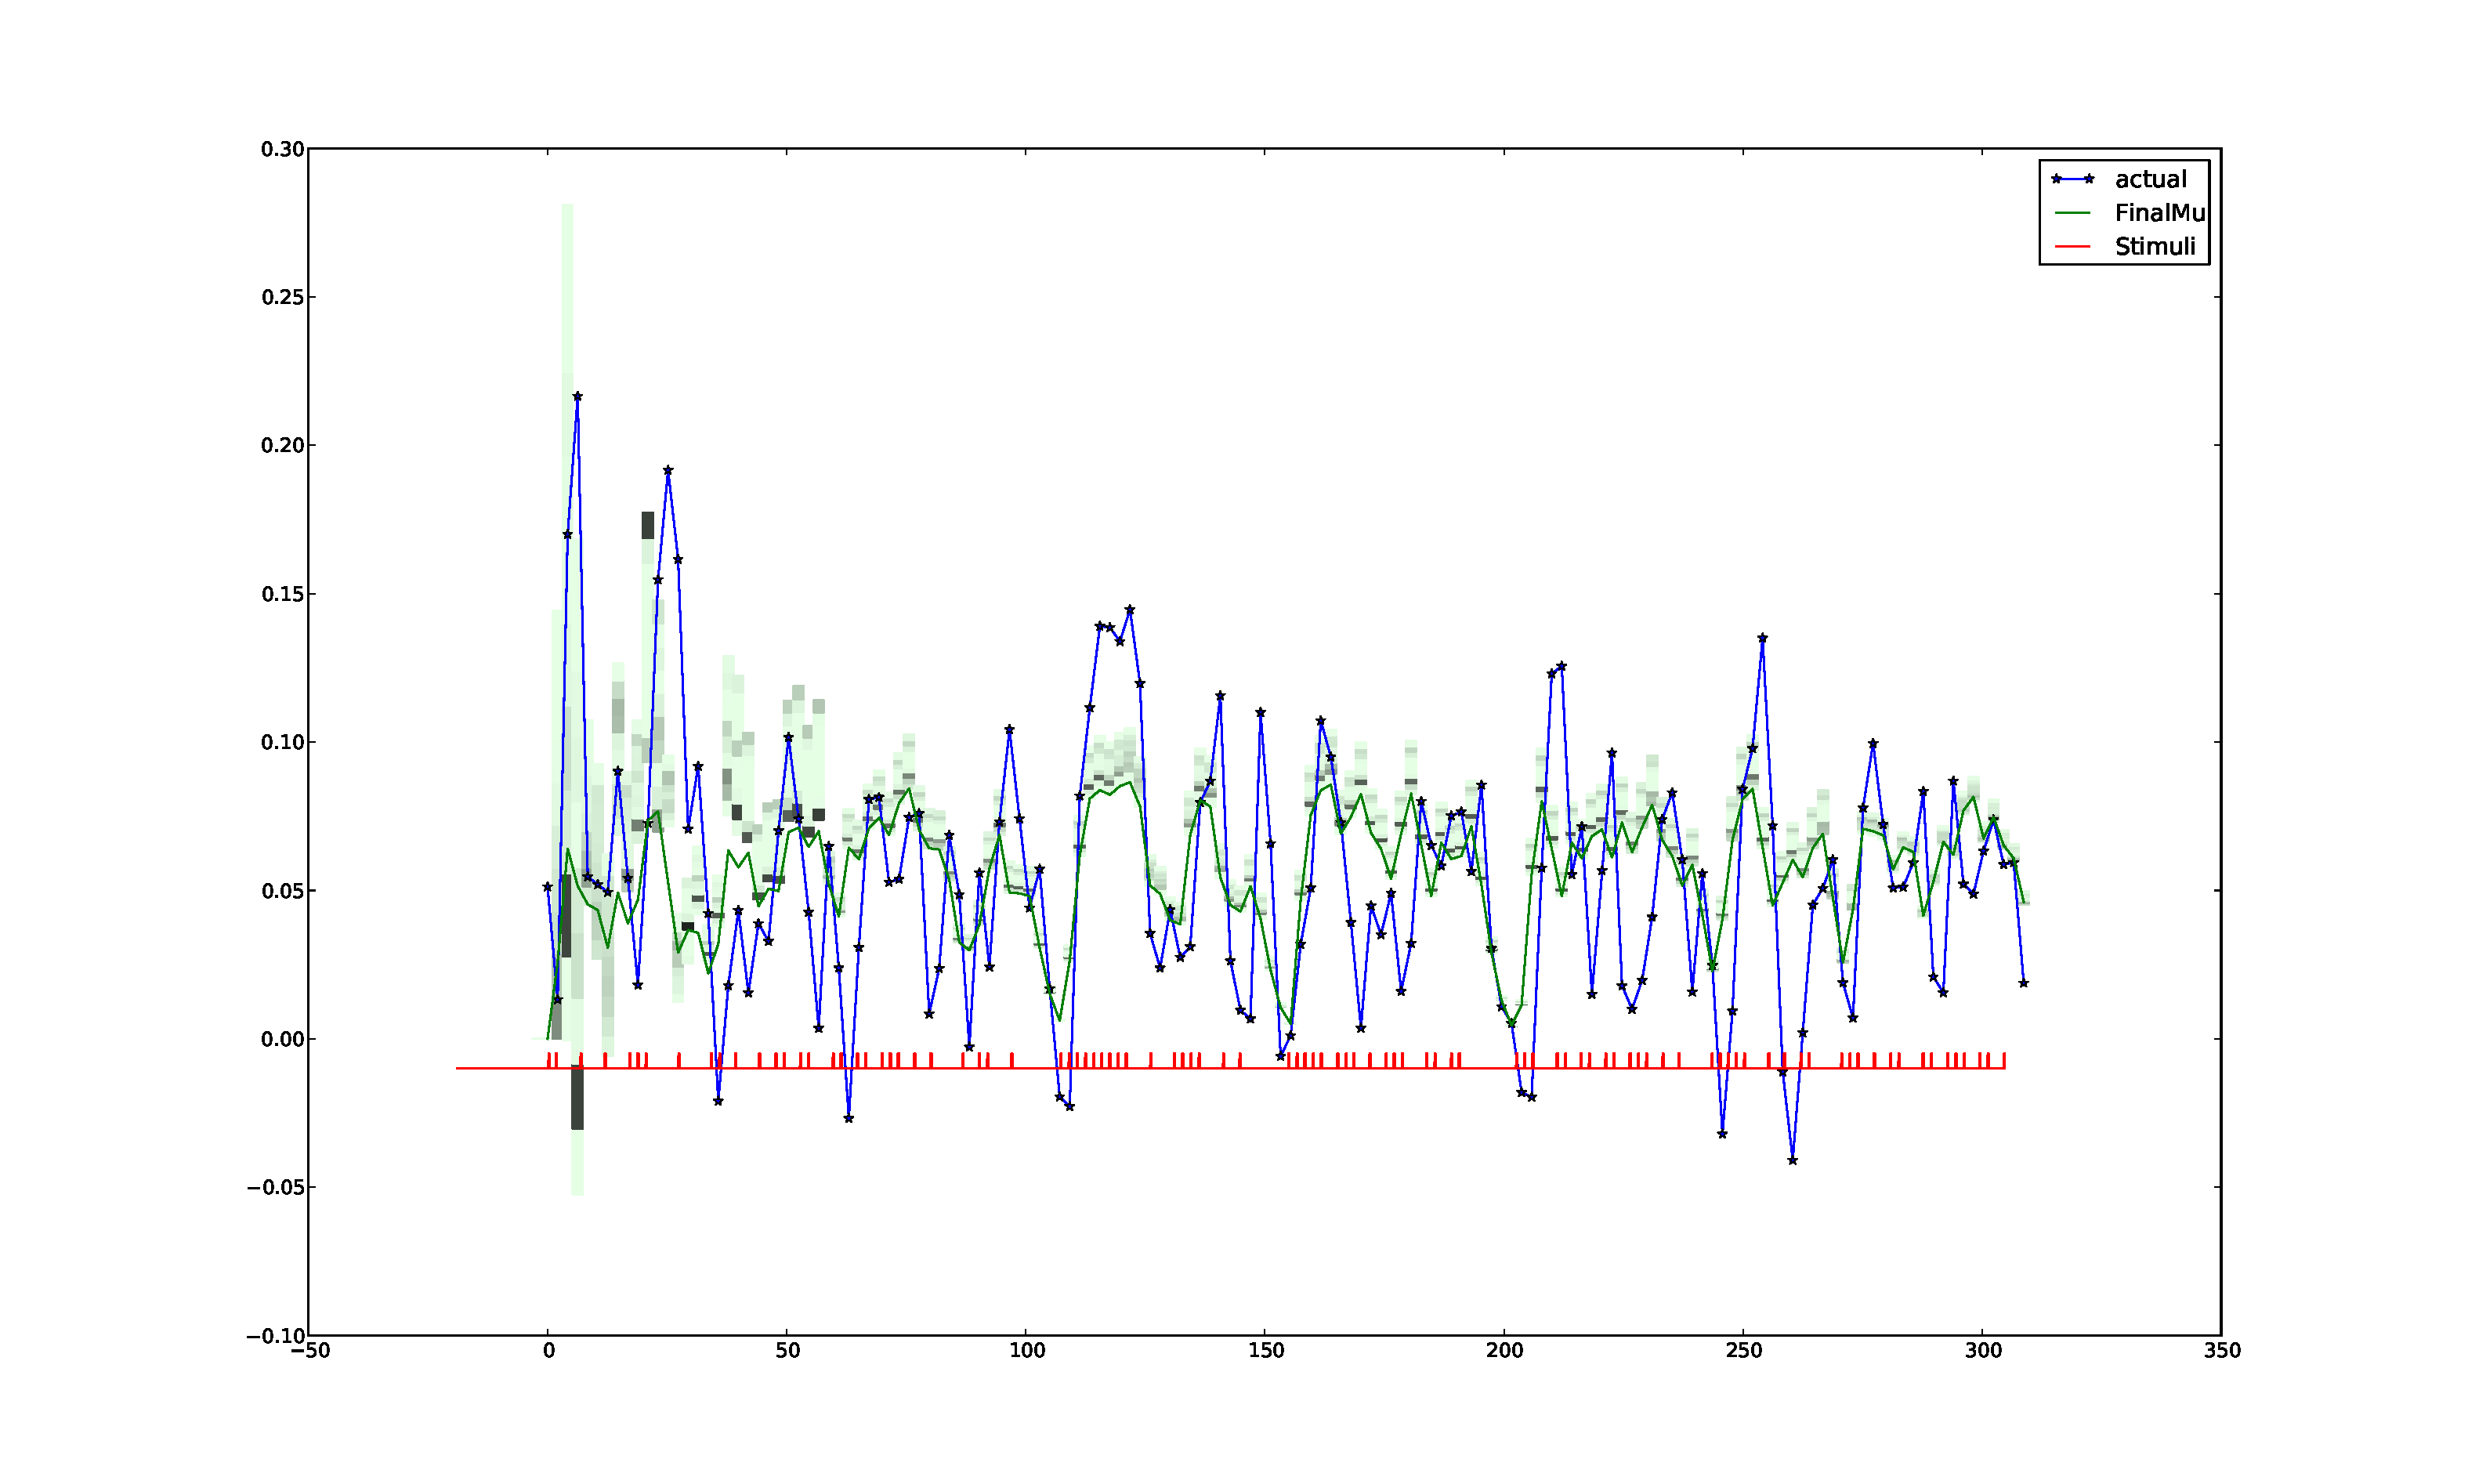
\includegraphics[clip=true,trim=10cm 4cm 10cm 4cm, width=16cm]{images/active_difficult}
\caption{Example of a timeseries that laplace performs better on than
gaussian. The large spike at the beginning can quickly eliminate all particles} 
\label{fig:highhard}

\end{figure}

For this reason, it is important to threshold based on the MSE, and the
impulse response. Naturally the MSE is intended to catch very voxels with a
very poor fit,
but like \autoref{fig:badfit}, the algorithm may have found a line
down the middle that gives a decent mean squared error. In this case
the excessive smoothing and low actual activation level will easily
be distinguished by finding the peak response to single short pulse. 

The choice of a prior, as discussed previously, is extremely important. While a
prior may have the potential to give good results, being a monte-carlo algorithm
there is the possibility for inconsistencies. Thus, increasing the variance
of the time-constants may allow additional flexibility, it will also cause
additional model variance. Case in point, the exact same algorithm run twice
with standard deviations of $.35, .35, .35$ for the time constants resulted in two
very different fits, see \autoref{fig:param1_var}.

\begin{figure}
\subfigure[]{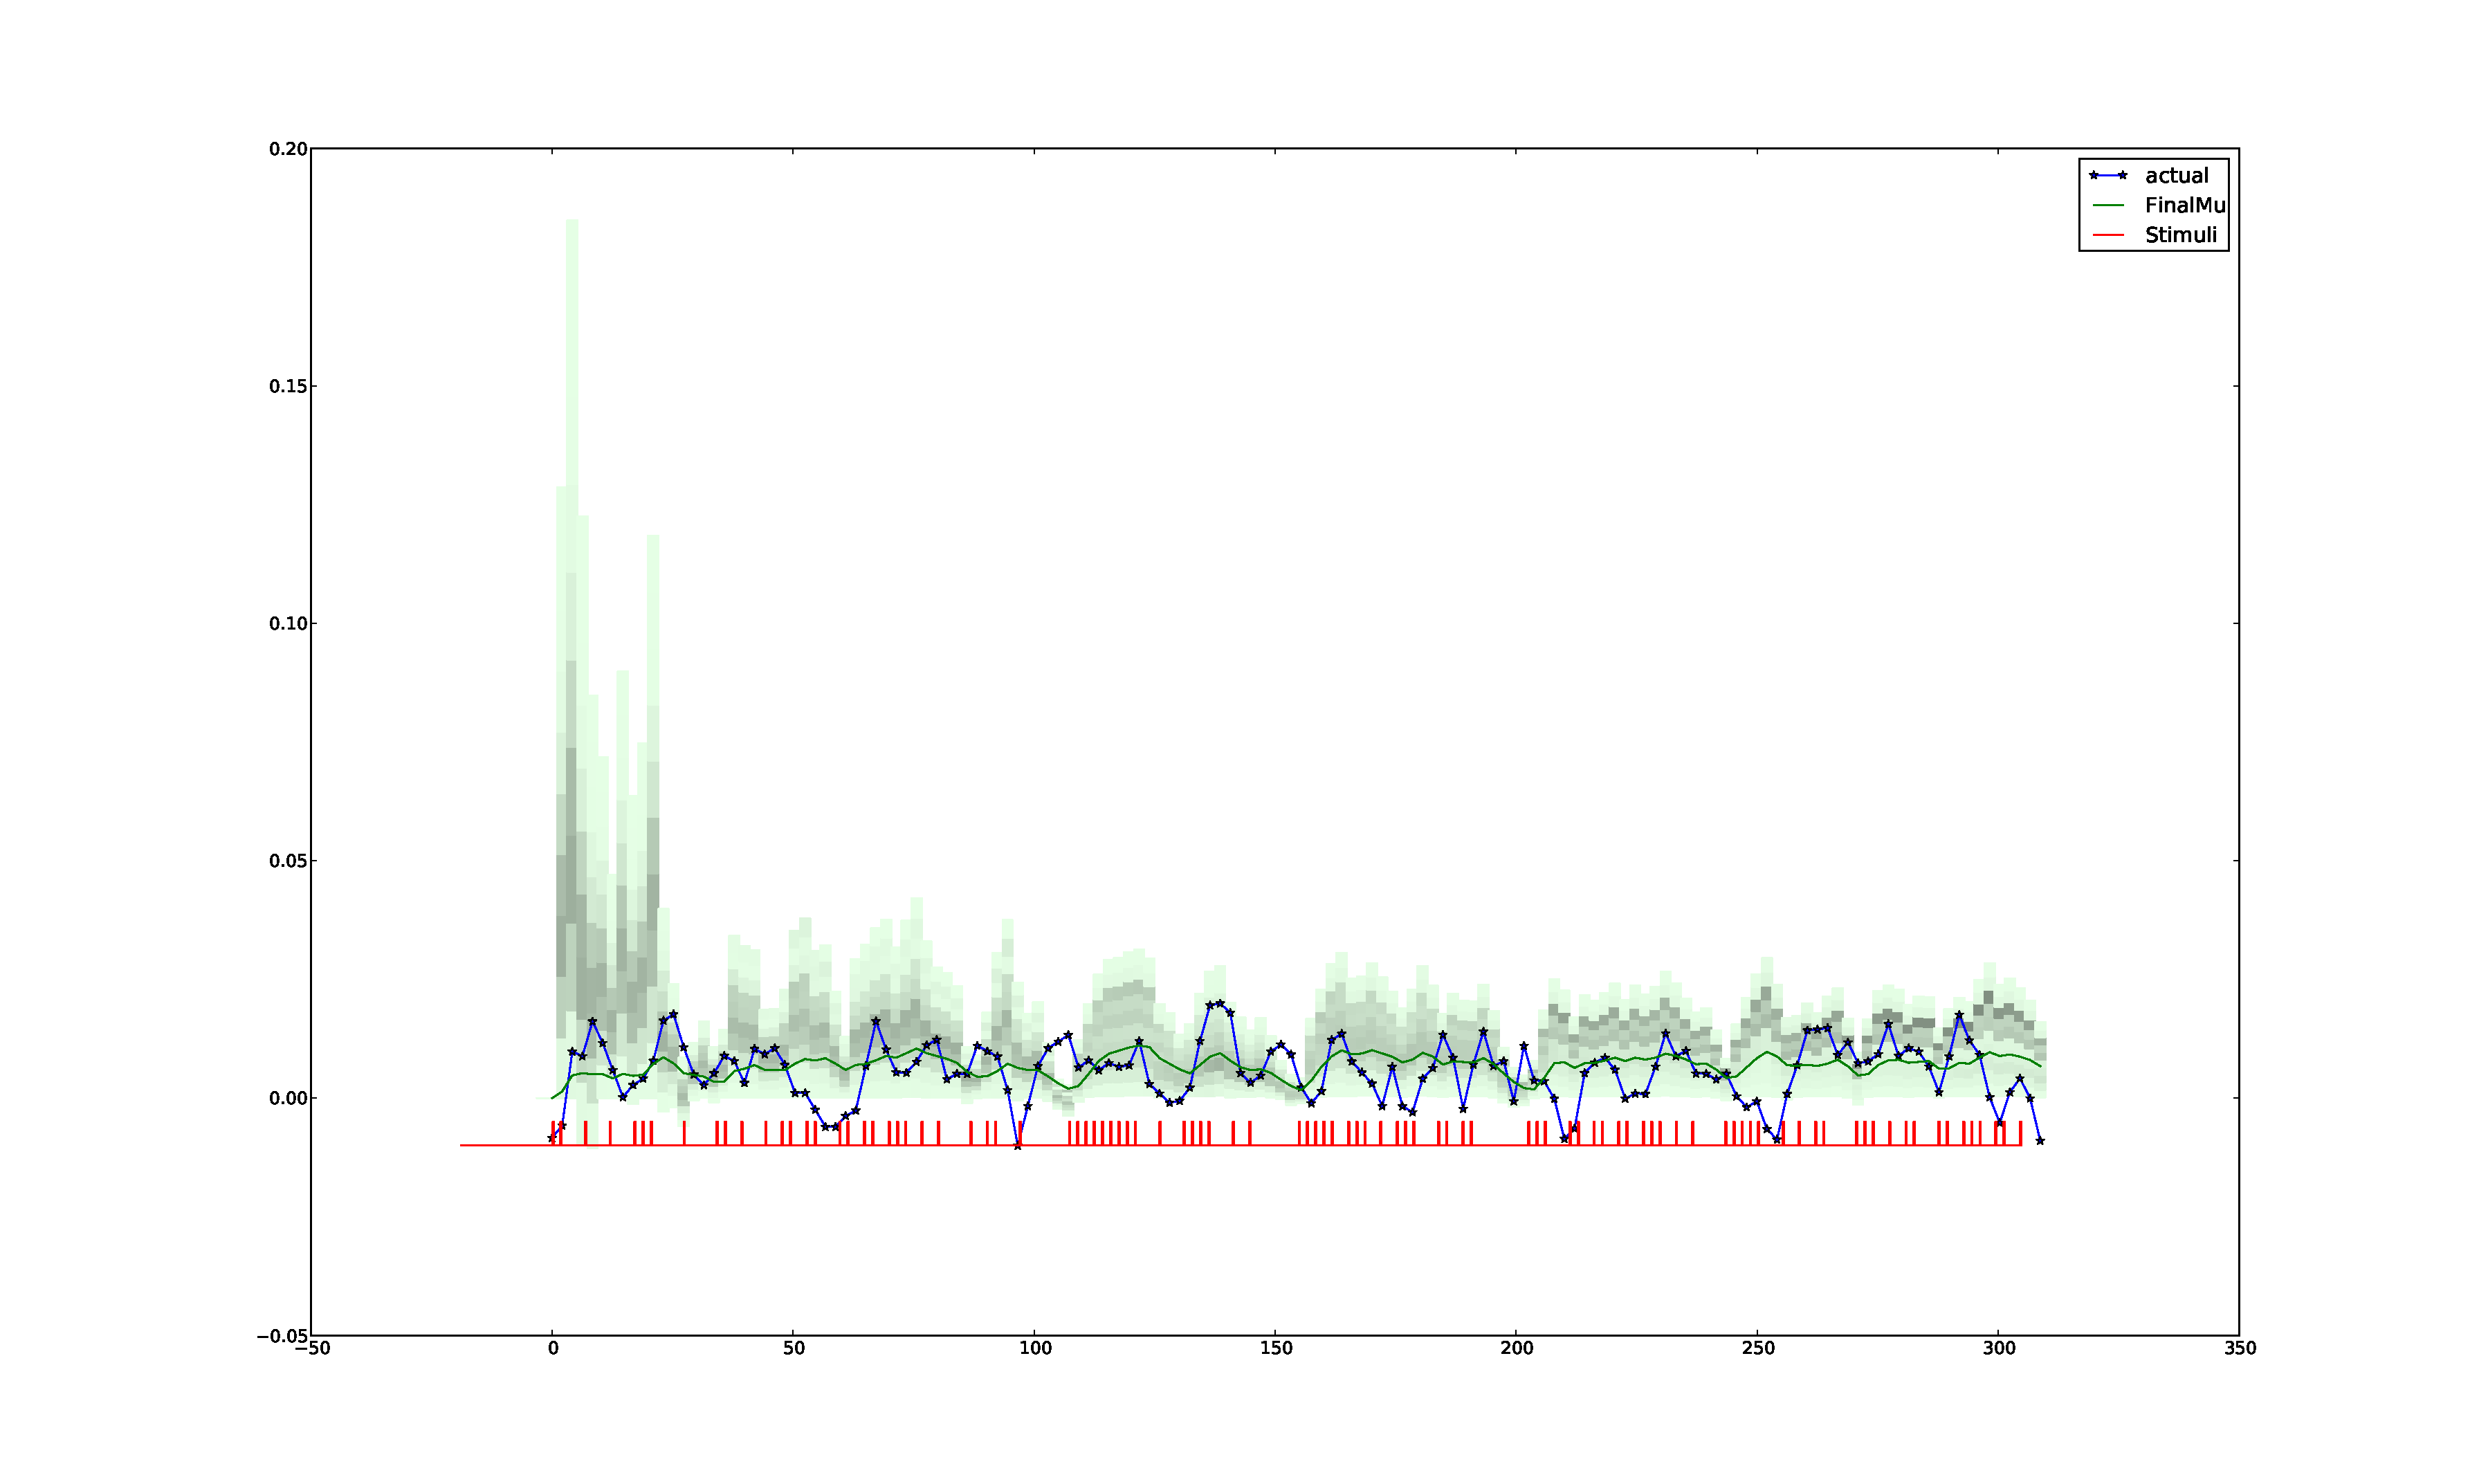
\includegraphics{images/badfit_param1}}
\subfigure[]{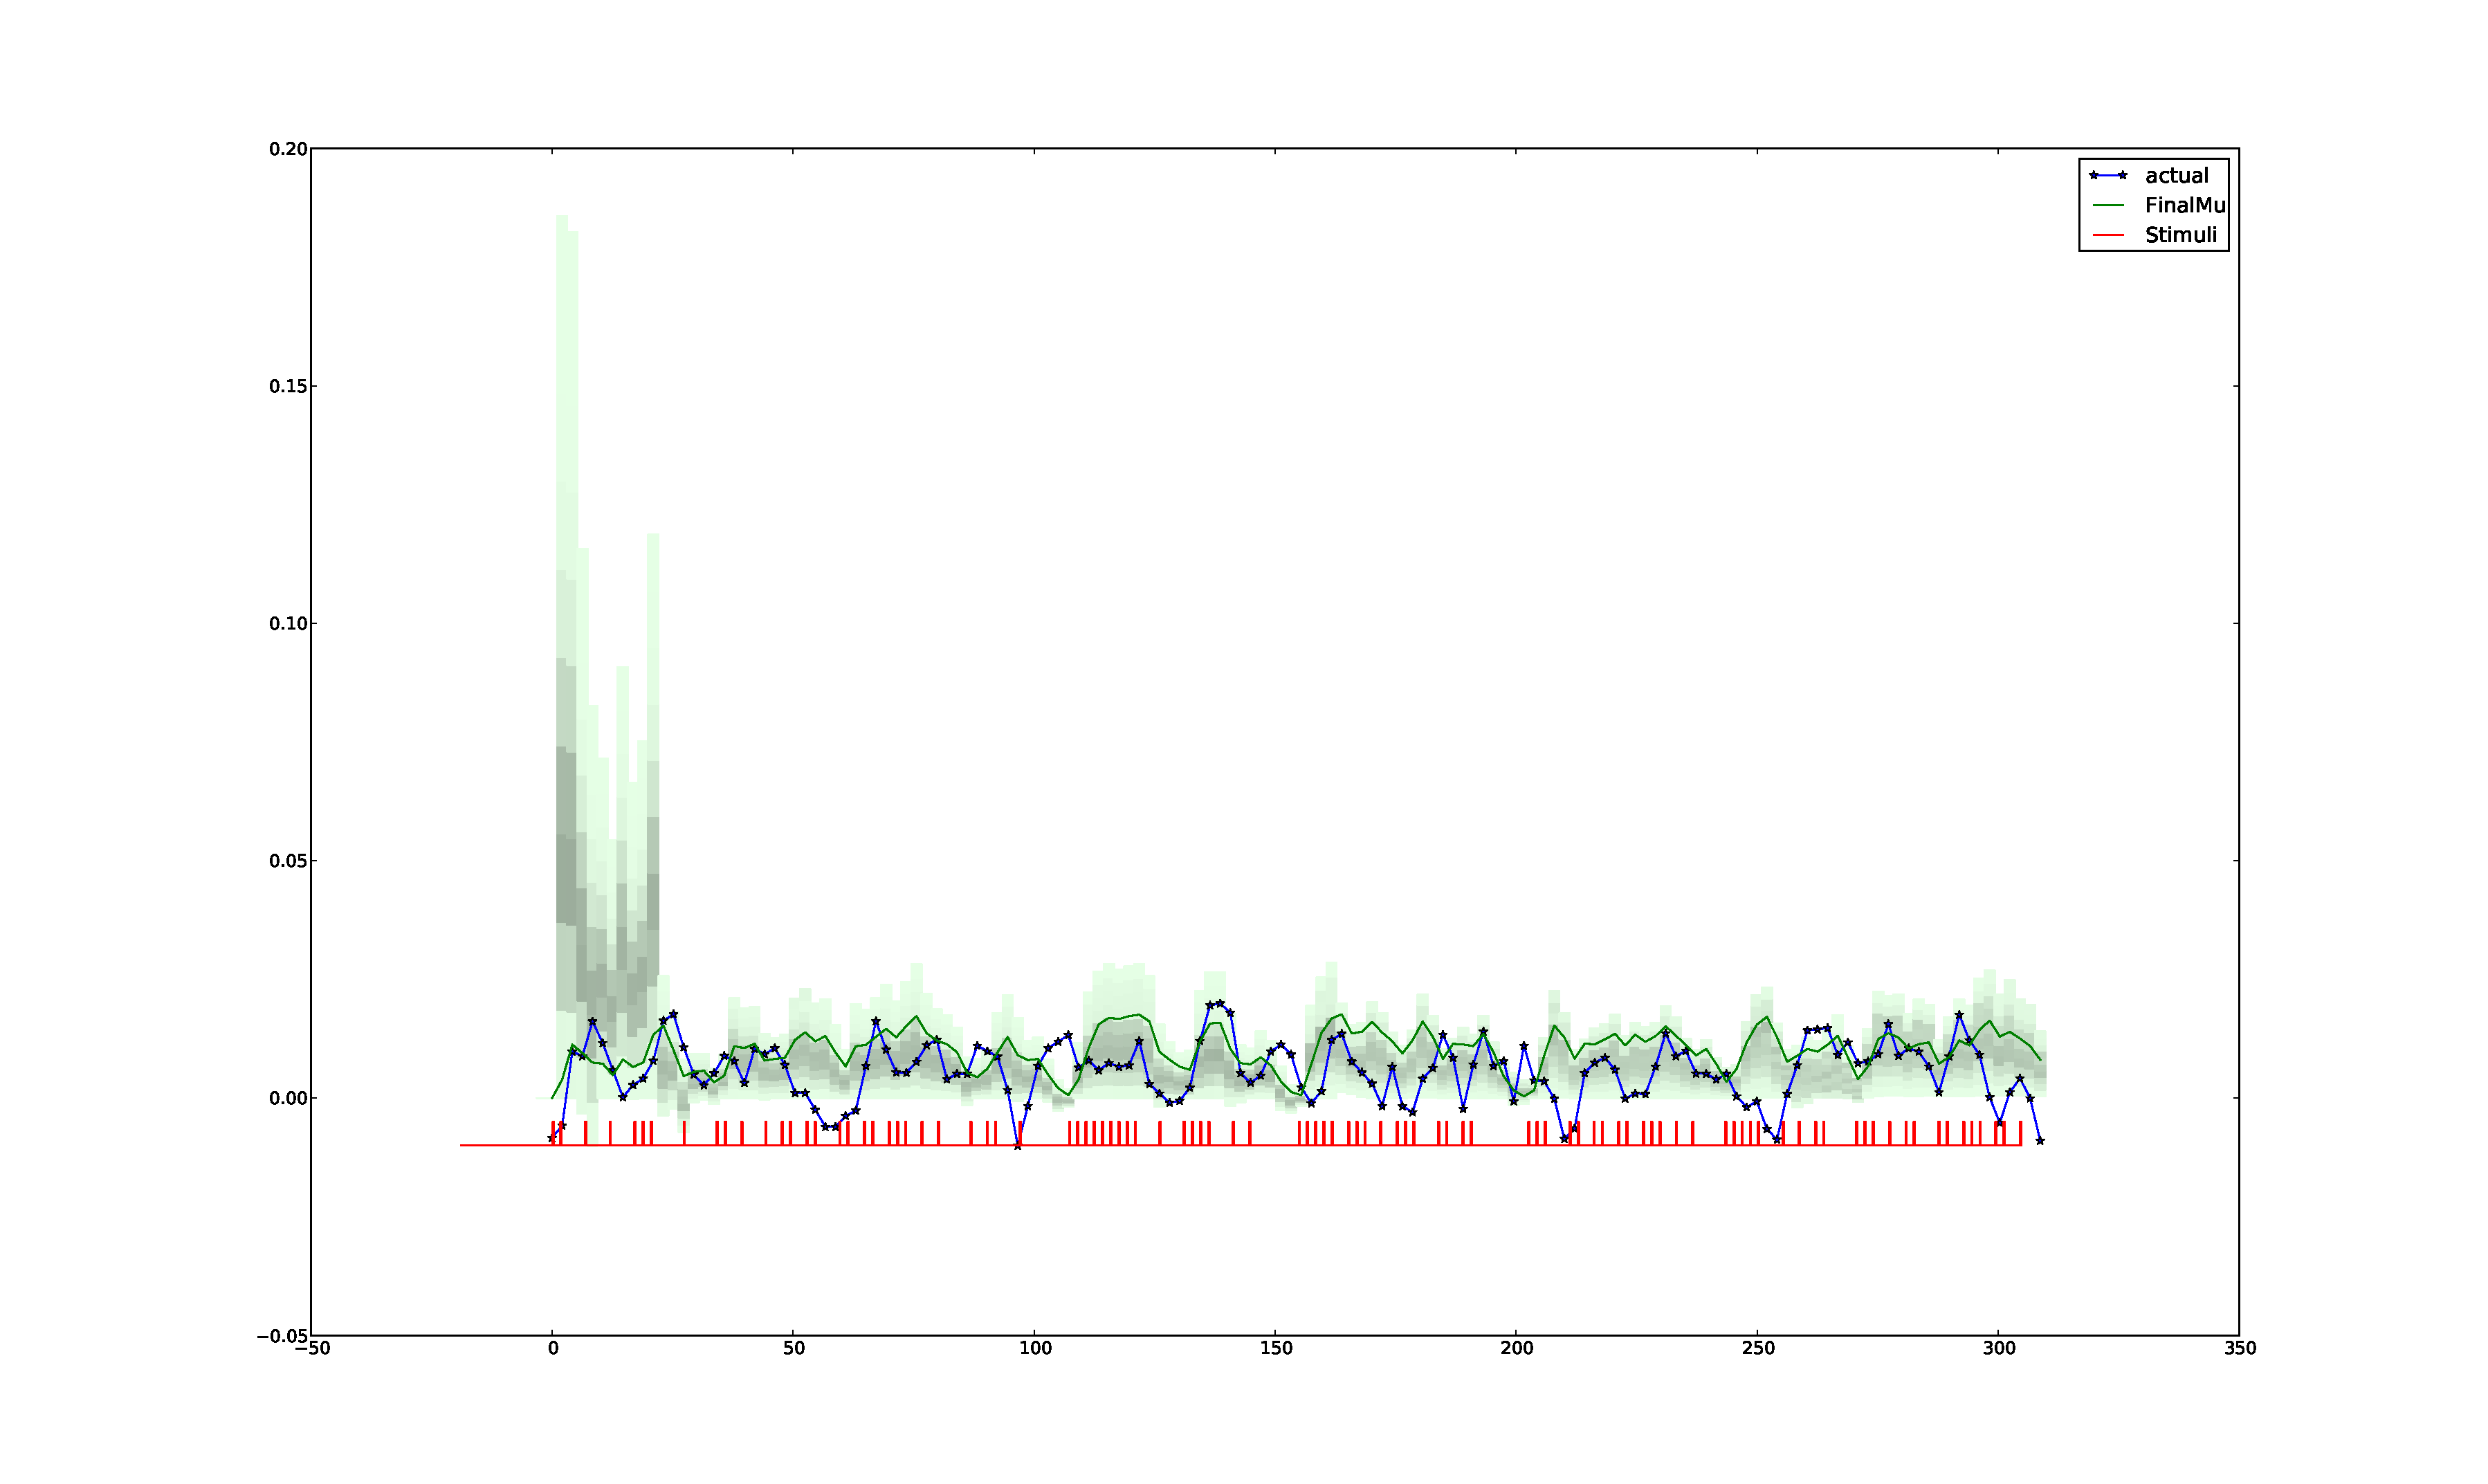
\includegraphics{images/goodfit_param1}}
\caption{The same priors gave rise to both fits. Params: ($\tau_0 \alpha E_0 V_0 \tau_f \tau_s \epsilon$)
for the good fit: $(1.40 .32 0.34 0.04  0.96 2.76)$, and for the poor fit:
$(2.28 0.32 0.33 0.017 0.67 2.88 1.36)$.}
\label{fig:badfit_param1}
\end{figure}

For this reason, I actually lowered the standard deviattions of the time
constants to prevent over-smoothing. This resulted in the more consistent, but
slightly worse results seen in \autoref{fig:param2_var}

\begin{figure}
\subfigure[]{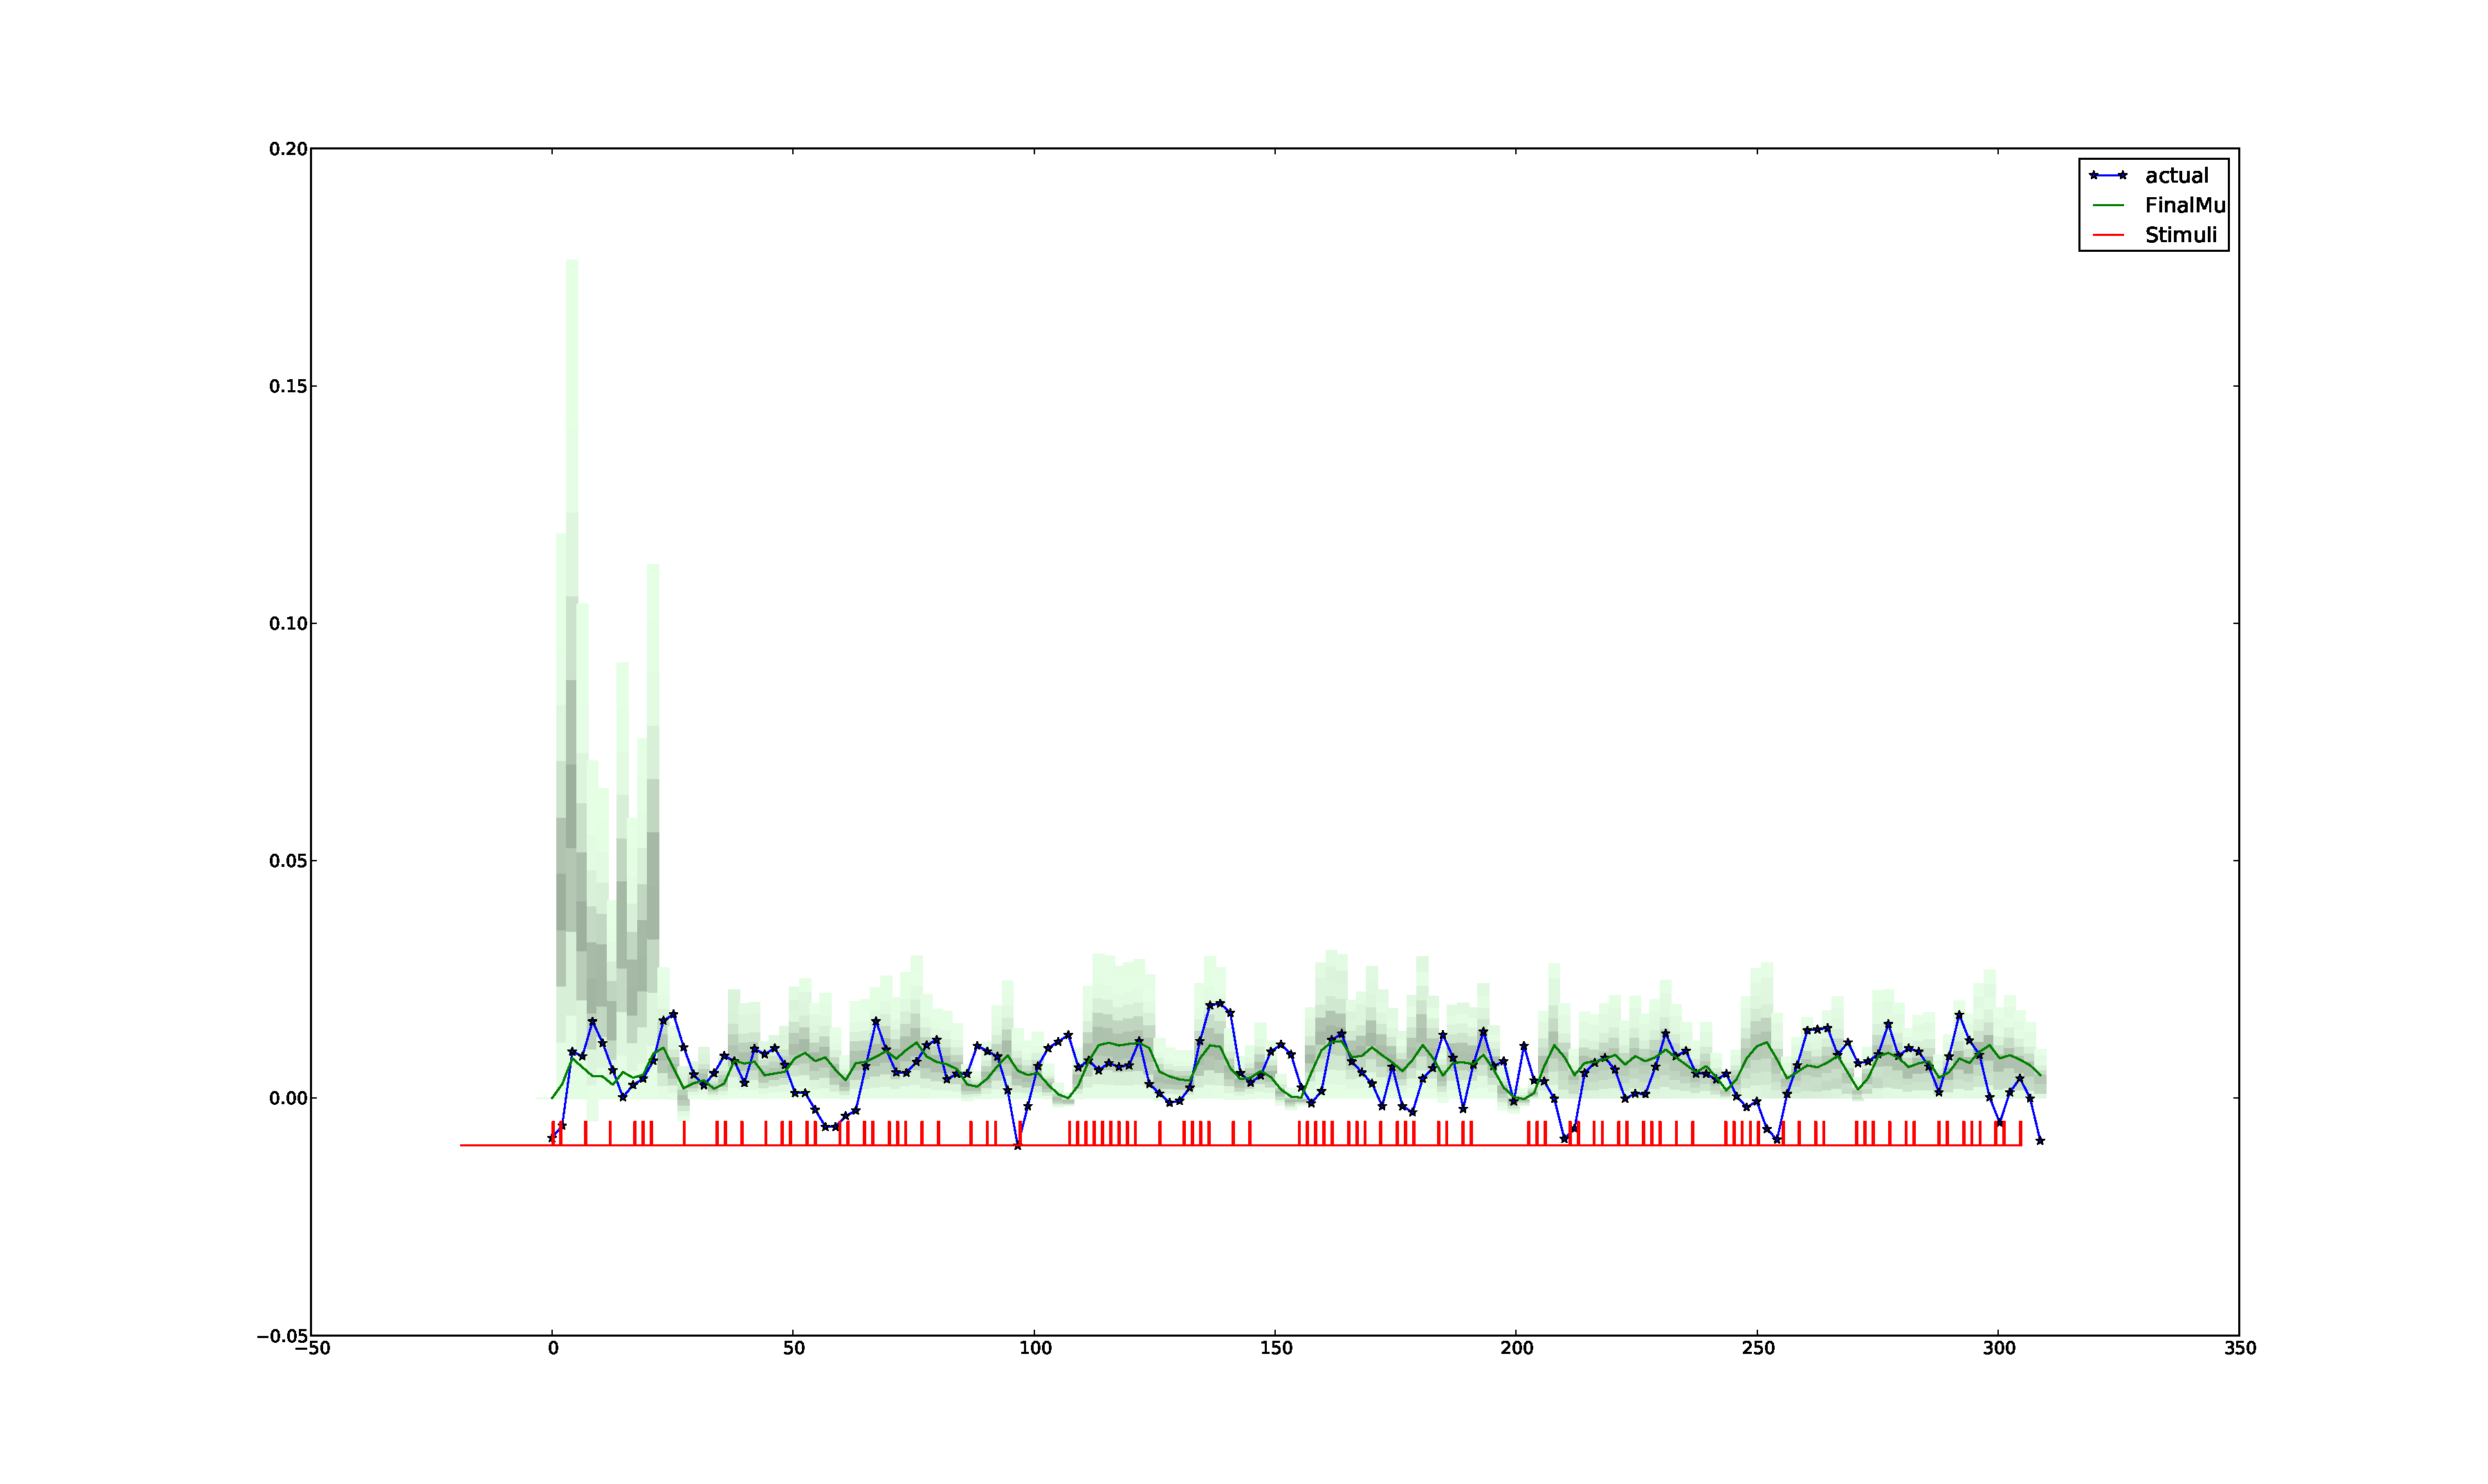
\includegraphics{images/param2a}}
\subfigure[]{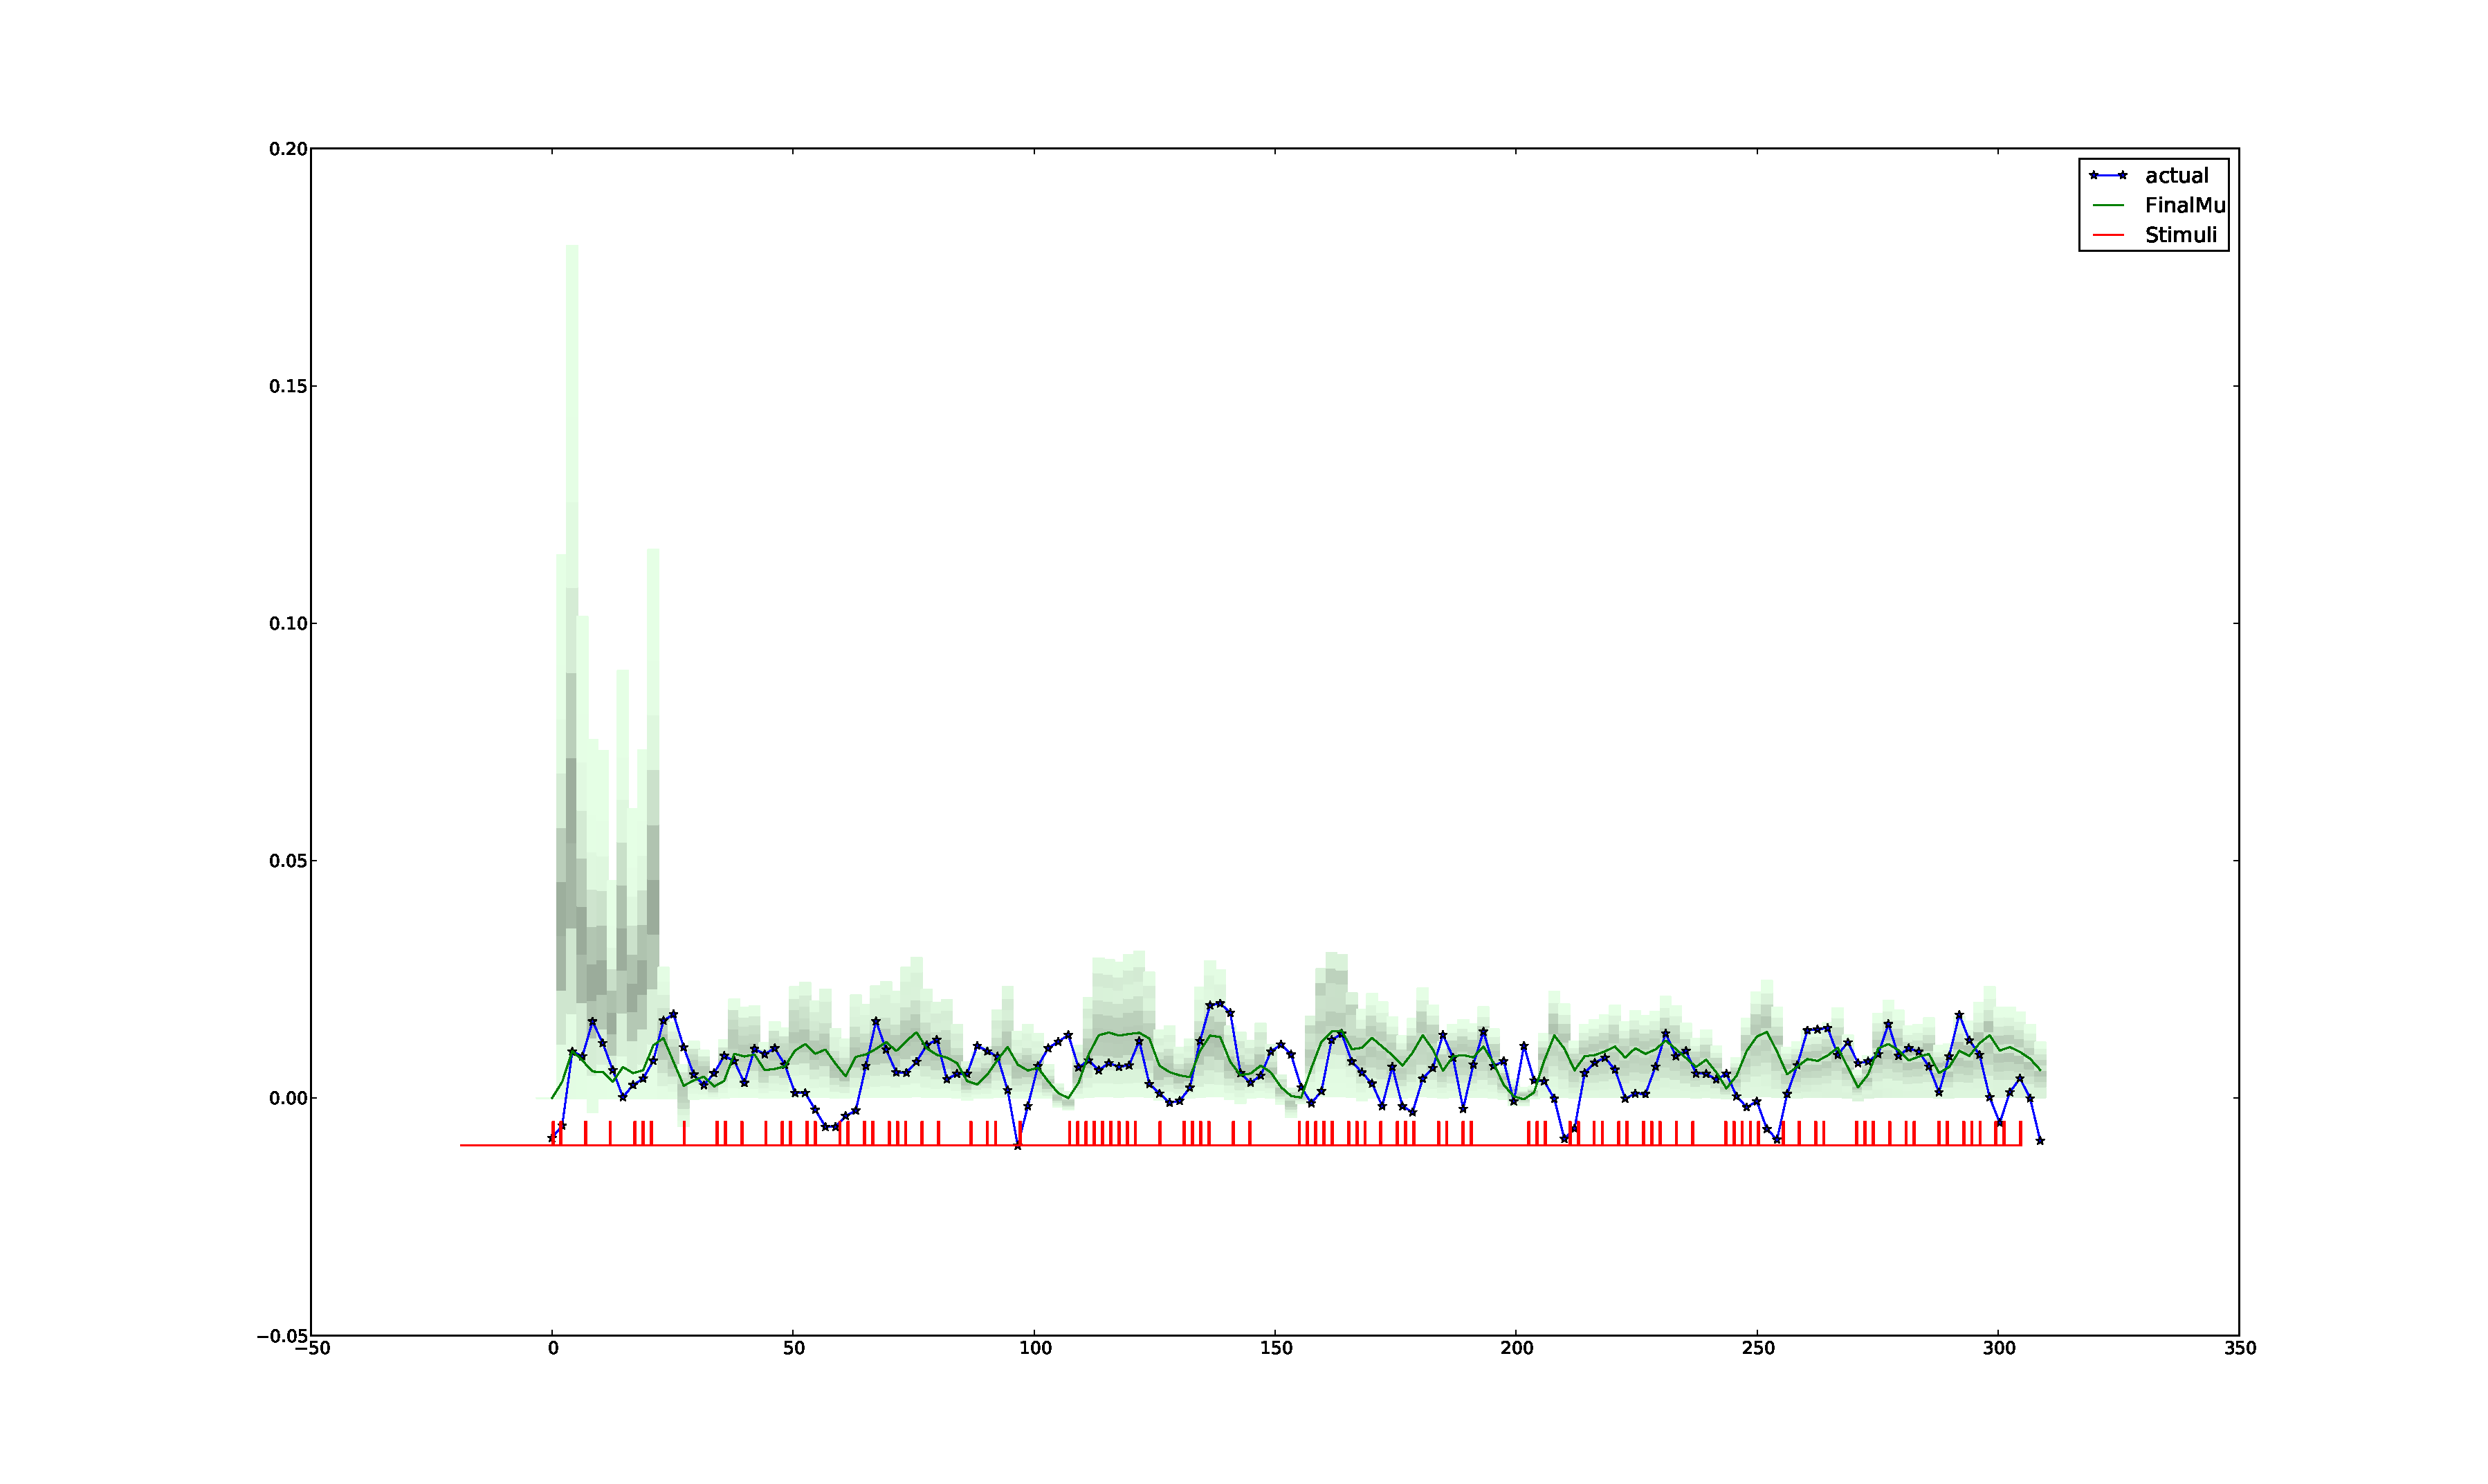
\includegraphics{images/param2b}}
\caption{A poor fit, using the same parameters as }
\label{fig:param2_var}
\end{figure}

\section{Particle Collapse Recovery}
This heuristic was initially intended to deal with cases where the particle
filter prematurely converged; and to reverse this effect. In reality, however
it did not perform well, and so it was not used in full-brain analysis. Ultimately
it did not prevent collapse of the distribution, and it often caused dramatic
increased in the variance of parameter estimates. It also pronged the analysis
time of inactive time series. Essentially the effect was exactly opposite of what
one would hope.


\section{Single Time-Series Simulation}

Graphs: 

For simulated data, single timeseries:

For \{delta, DC/Spline\}, \{exponential, gaussian, cauchy\}, \{biased, unbiased initial\},
\{100, 500, 1000\} particles
\begin{enumerate}
\item Ground truth vs. Estimated signal during particle filter run
\item Ground truth vs. Estimated signal with final parameter set
\item True Parameters vs. Final Parameter Sets
\item Variance of final parameters when faced with same ground truth, different noise
\item MSE of (a new timeseries based on X(t) vs. ground truth) for all t
\item Estimator Variance based on different noise runs
\item Final Particle Distribution
\end{enumerate}

For Simulated Data, Full Volume:

%note to self, epsilon should probably be uniform between 0 and something
\section{Simulated Volume}

\chapter{Real Data}
\begin{figure}
\subfigure[]{\label{fig:hm_spm} 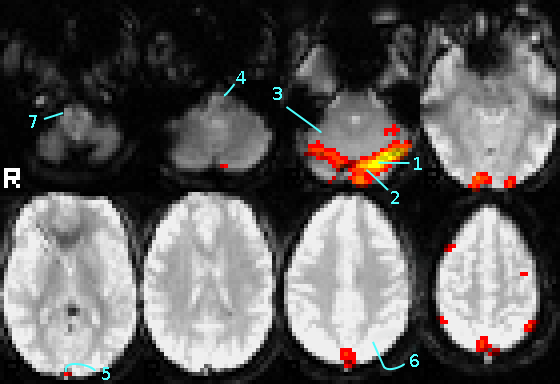
\includegraphics[scale=.66]{images/spm_hm}}
\subfigure[]{\label{fig:hm_canon_spm_x} 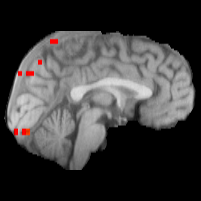
\includegraphics[scale=.85]{images/spm_hm_x}}
\subfigure[]{\label{fig:hm_canon_spm_y} 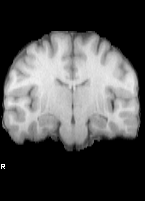
\includegraphics[scale=.85]{images/spm_hm_y}}
\subfigure[]{\label{fig:hm_canon_spm_z} 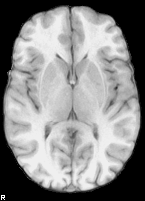
\includegraphics[scale=.85]{images/spm_hm_z}}
\subfigure{\label{fig:scale_spm} 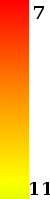
\includegraphics[scale=.3]{images/scale1}}
\caption{Sagittal, coronal and axial slices of SPM results (\autoref{fig:hm_canon_spm_x} \autoref{fig:hm_canon_spm_y} 
         \autoref{fig:hm_canon_spm_x}), as well as a series of axial slices, \autoref{fig:hm_spm}. Units
         of activation are in Student's T-scores. Higher indicates higher assurance that the signal cannot
         have occurred through noise alone.}
\label{fig:hm_canon_spm}
\end{figure}

\begin{figure}
\subfigure[]{\label{fig:hm_pfilter} 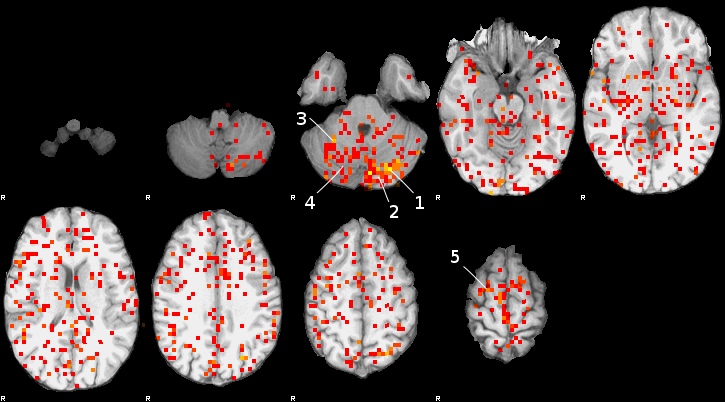
\includegraphics[scale=.66]{images/pfilter_hm}}
\subfigure[]{\label{fig:hm_canon_pfilter_x} 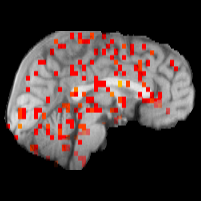
\includegraphics[scale=.85]{images/pfilter_hm_x}}
\subfigure[]{\label{fig:hm_canon_pfilter_y} 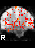
\includegraphics[scale=.85]{images/pfilter_hm_y}}
\subfigure[]{\label{fig:hm_canon_pfilter_z} 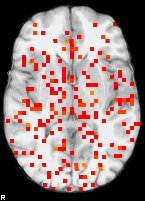
\includegraphics[scale=.85]{images/pfilter_hm_z}}
\subfigure{\label{fig:scale_pfilter} 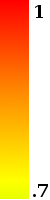
\includegraphics[scale=.3]{images/scale2}}
\caption{Sagittal, coronal and axial slices of SPM results (\autoref{fig:hm_canon_pfilter_x} \autoref{fig:hm_canon_pfilter_y} 
         \autoref{fig:hm_canon_pfilter_x}), as well as a series of axial slices, \autoref{fig:hm_pfilter}. 
         Units of match is normalized $\sqrt{MSE}$. The lowest (best) levels were $.7$,
         whereas the worst levels could go higher than 100 (not shown).}
\label{fig:hm_canon_pfilter}
\end{figure}

\begin{figure}
\subfigure[]{\label{fig:hm_pfilter85} 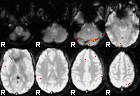
\includegraphics[scale=.66]{images/pfilter85_hm}}
\subfigure[]{\label{fig:hm_canon_pfilter85_x} 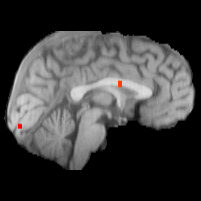
\includegraphics[scale=.85]{images/pfilter_hm85_x}}
\subfigure[]{\label{fig:hm_canon_pfilter85_y} 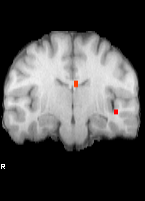
\includegraphics[scale=.85]{images/pfilter_hm85_y}}
\subfigure[]{\label{fig:hm_canon_pfilter85_z} 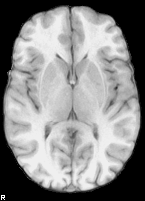
\includegraphics[scale=.85]{images/pfilter_hm85_z}}
\subfigure{\label{fig:scale_pfilter85} 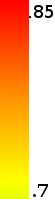
\includegraphics[scale=.3]{images/scale3}}
\caption{Sagittal, coronal and axial slices of SPM results (\autoref{fig:hm_canon_pfilter_x} \autoref{fig:hm_canon_pfilter_y} 
         \autoref{fig:hm_canon_pfilter_x}), as well as a series of axial slices, \autoref{fig:hm_pfilter}. 
         Units of match is normalized $\sqrt{MSE}$. The lowest (best) levels were $.7$,
         whereas the worst levels could go higher than 100 (not shown).}
\label{fig:hm_canon_pfilter85}
\end{figure}

\begin{figure}
\subfigure[Particle Filter]{\label{fig:comp1pfilter} 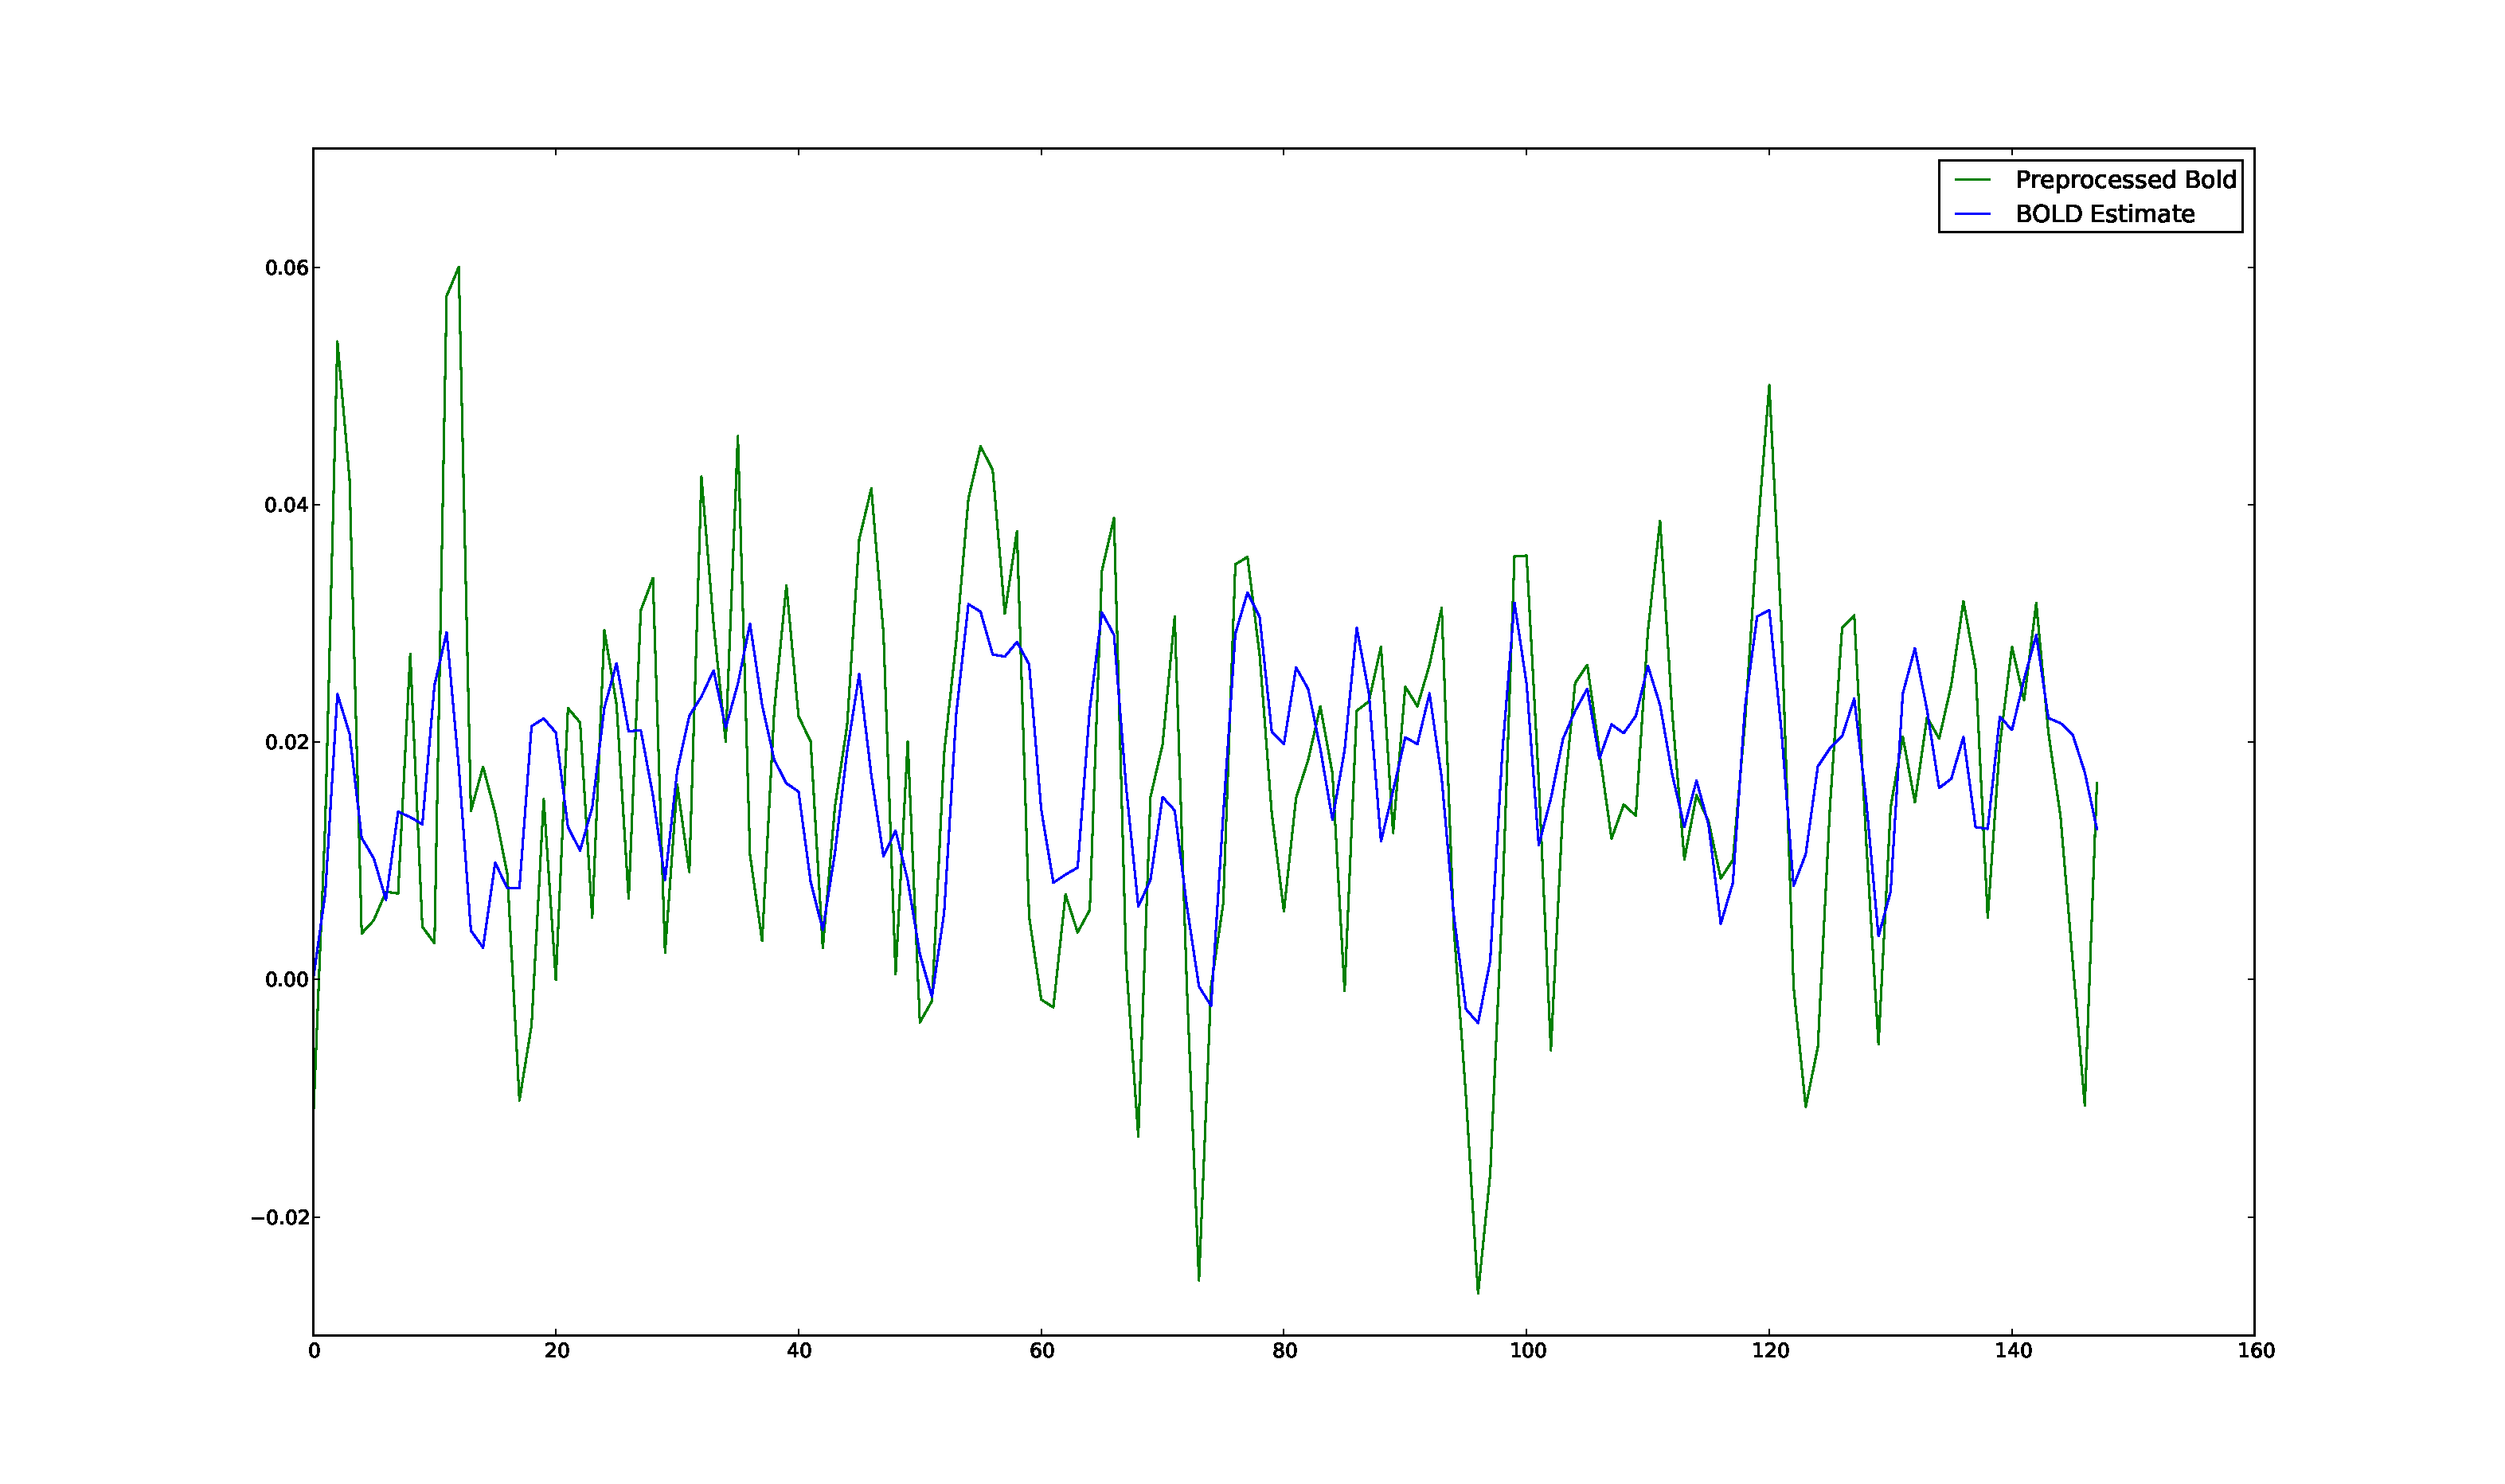
\includegraphics[clip=true,trim=5cm 1cm 4cm 1cm,width=15cm]{images/1_pfilter_37_14_7}}\\
\subfigure[SPM]{\label{fig:comp1spm} 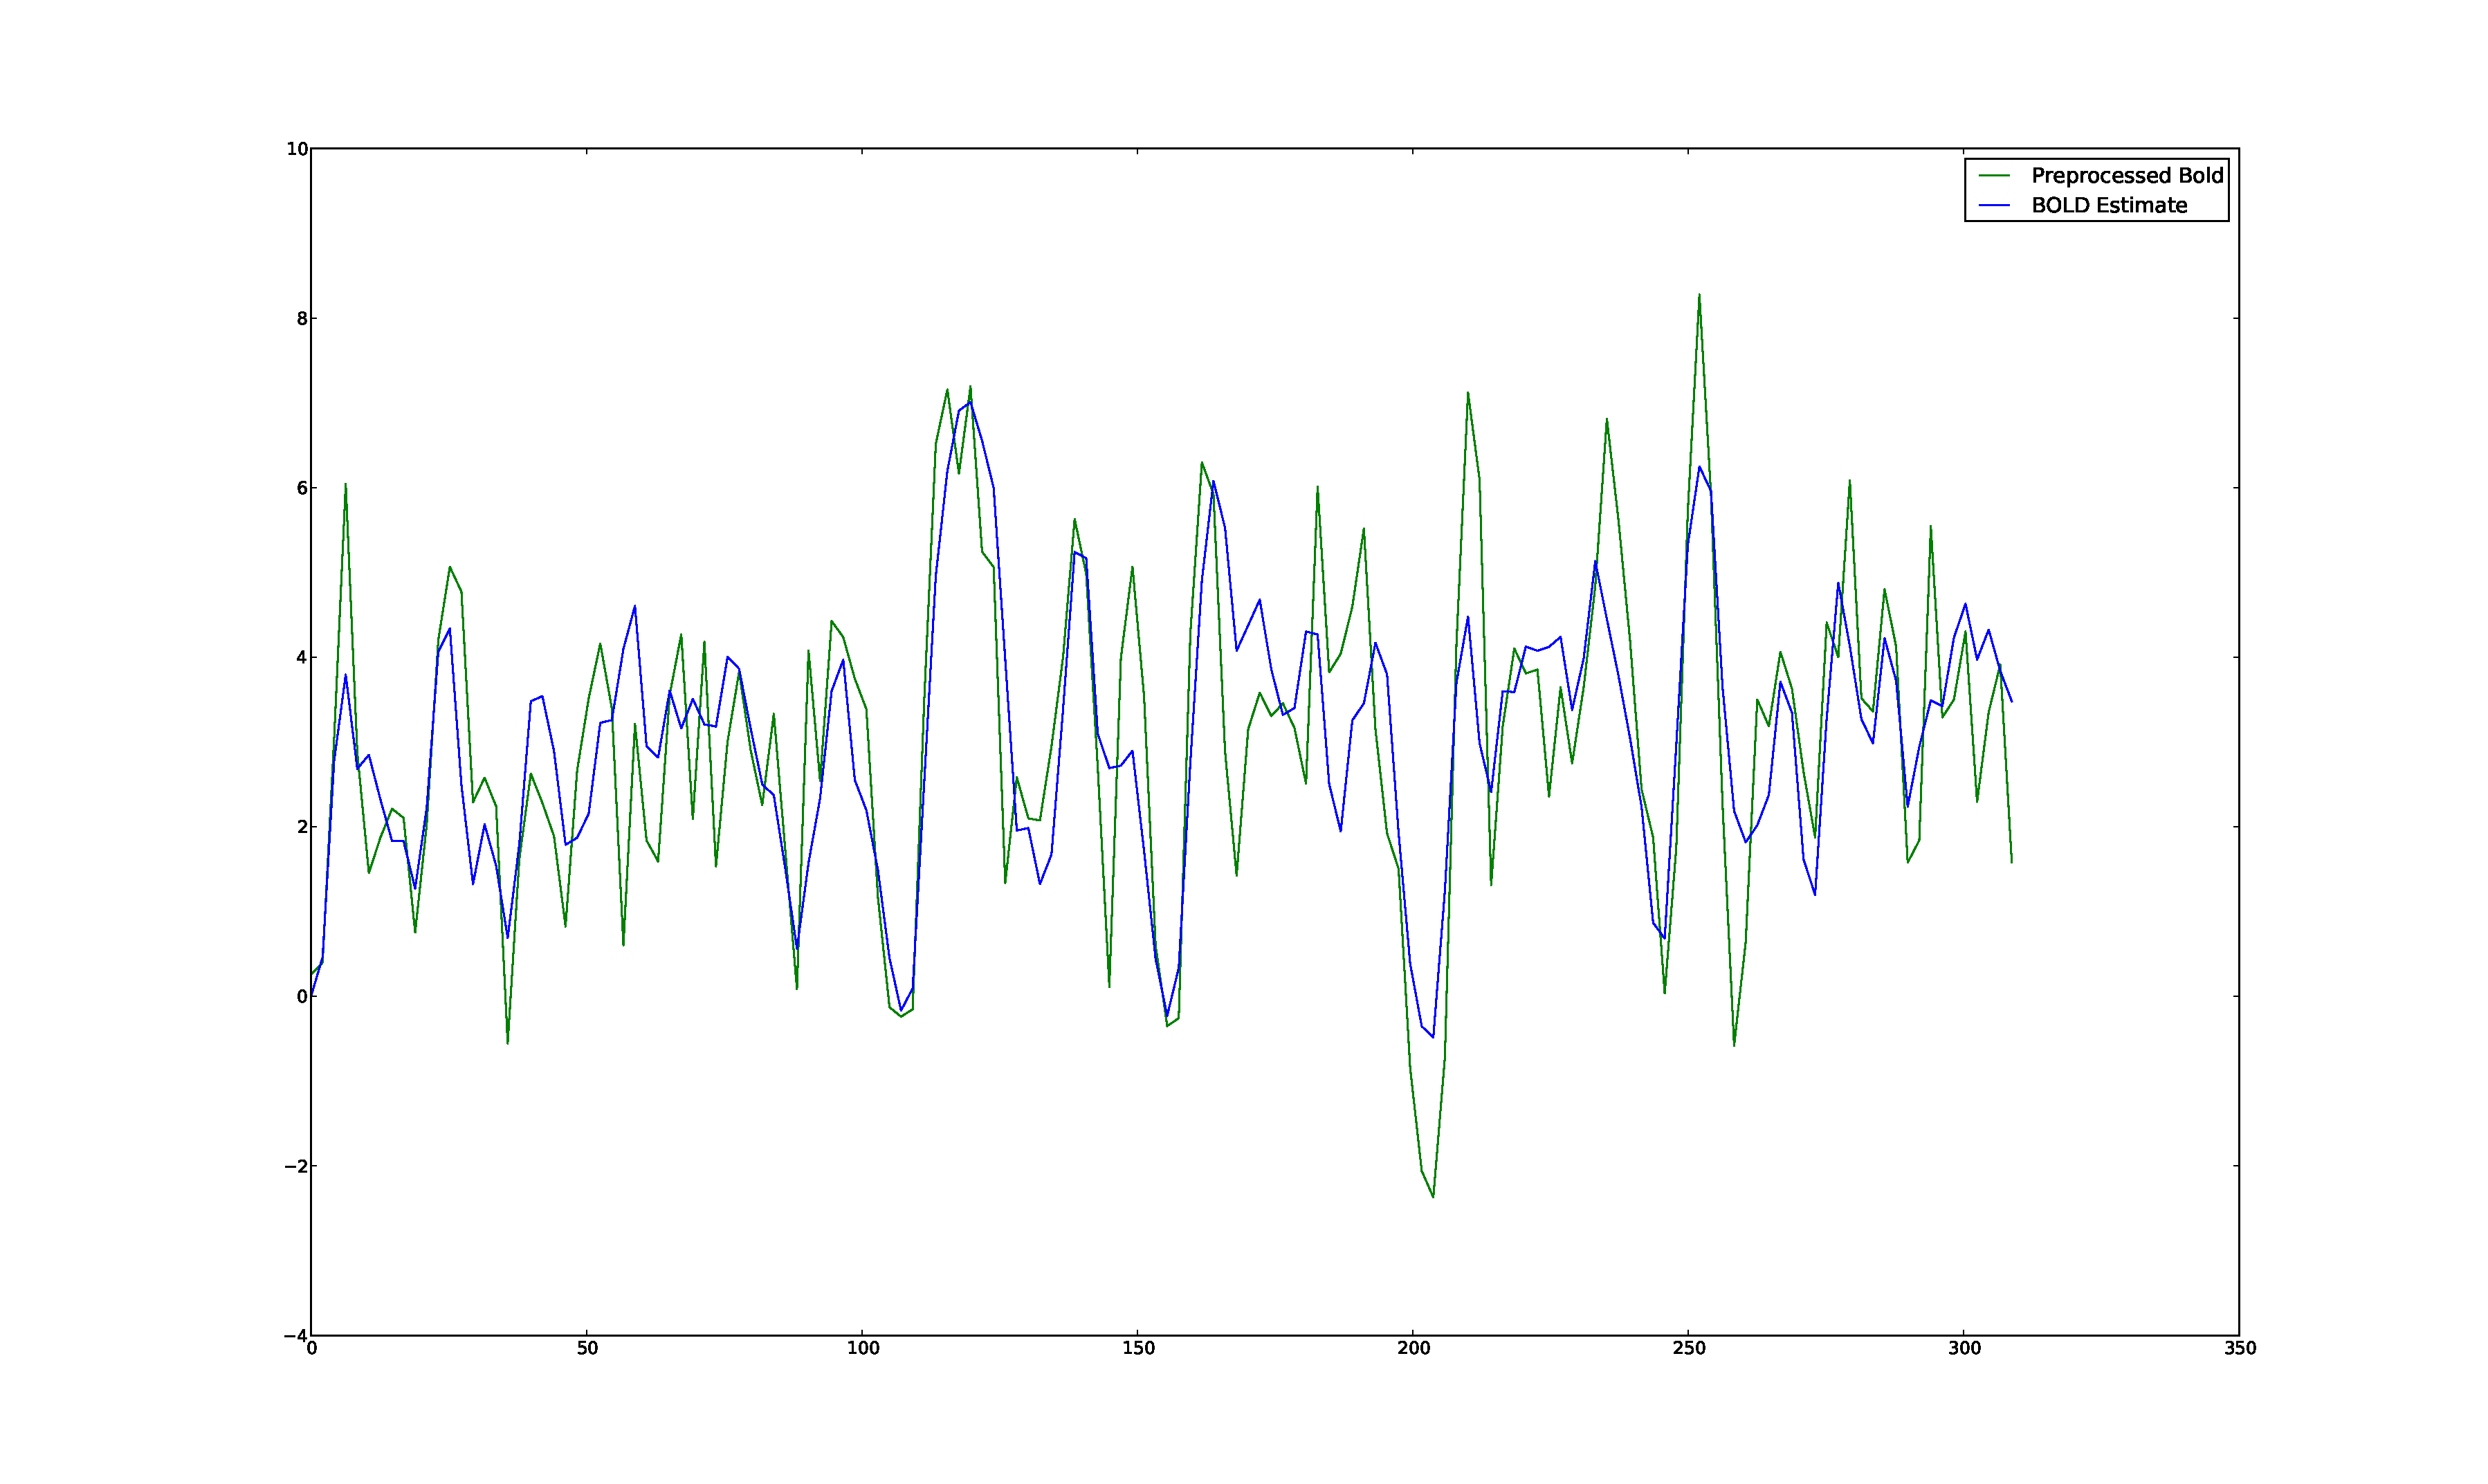
\includegraphics[clip=true,trim=5cm 1cm 4cm 1cm,width=15cm]{images/1_spm_37_14_7}}
\caption{}
\label{fig:comp1}
\end{figure}

\begin{figure}
\subfigure[Particle Filter]{\label{fig:comp2pfilter} 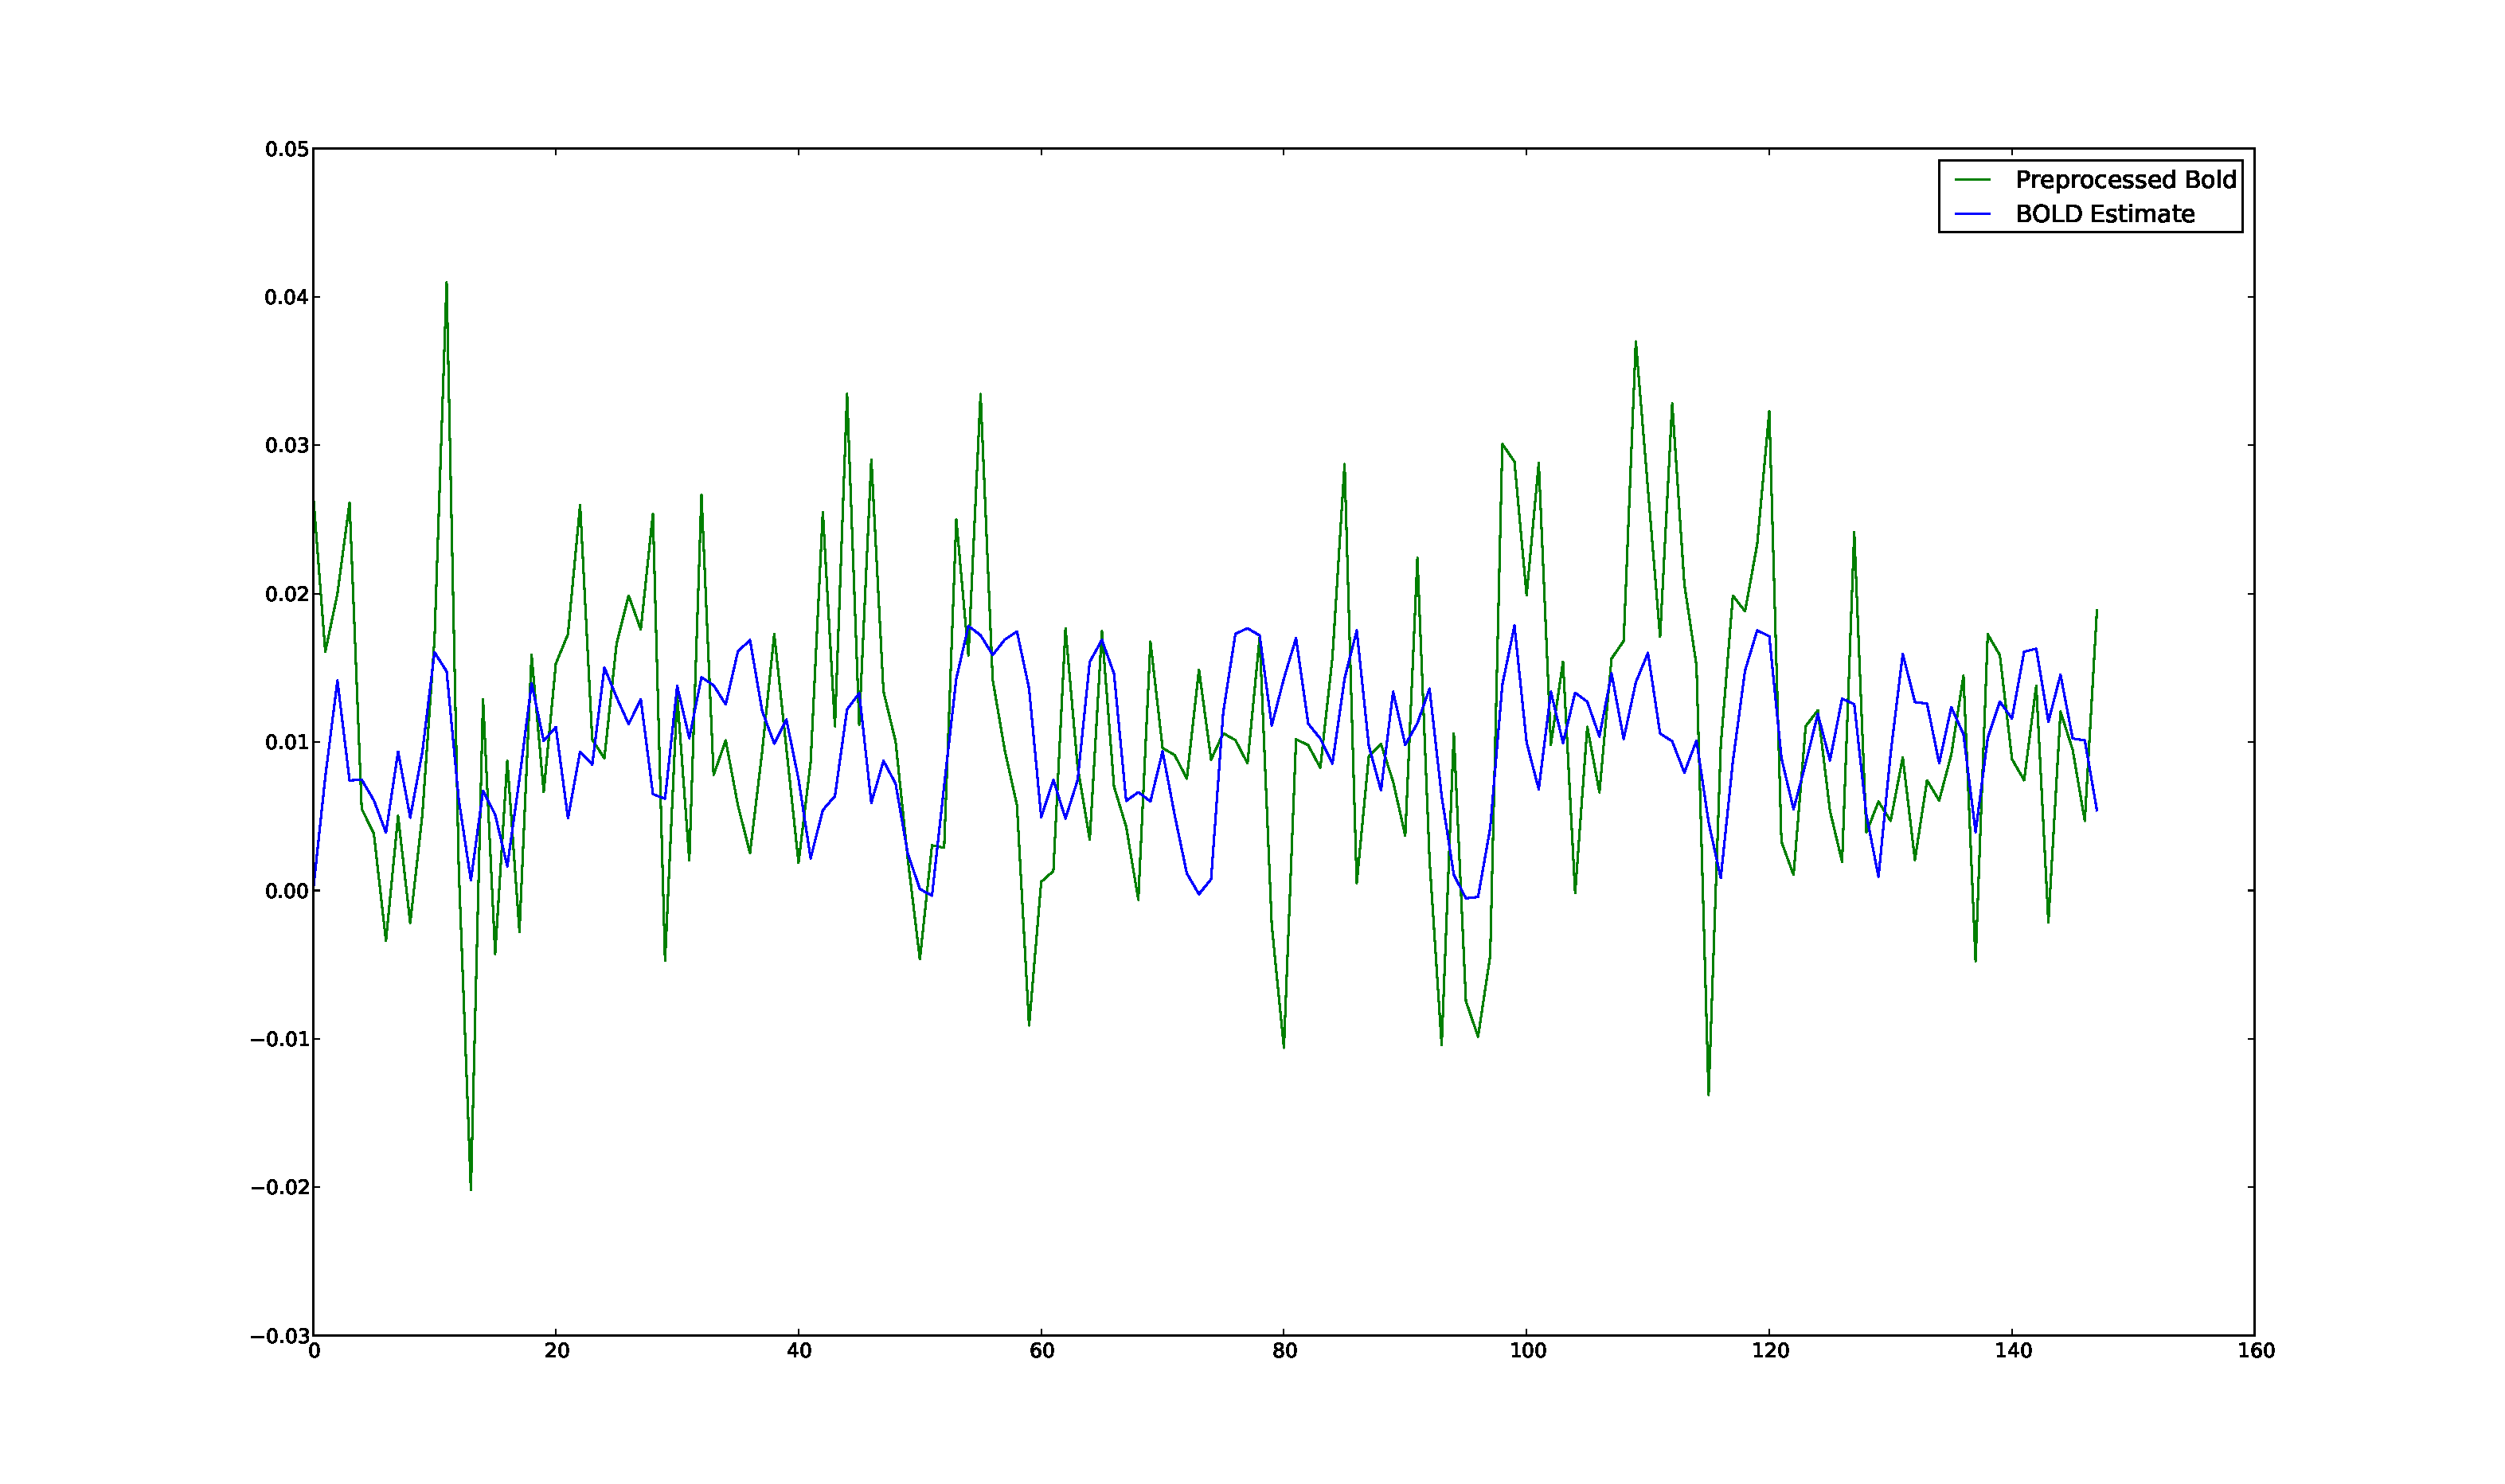
\includegraphics[clip=true,trim=5cm 1cm 4cm 1cm,width=15cm]{images/2_pfilter_34_12_7}}\\
\subfigure[SPM]{\label{fig:comp2spm} 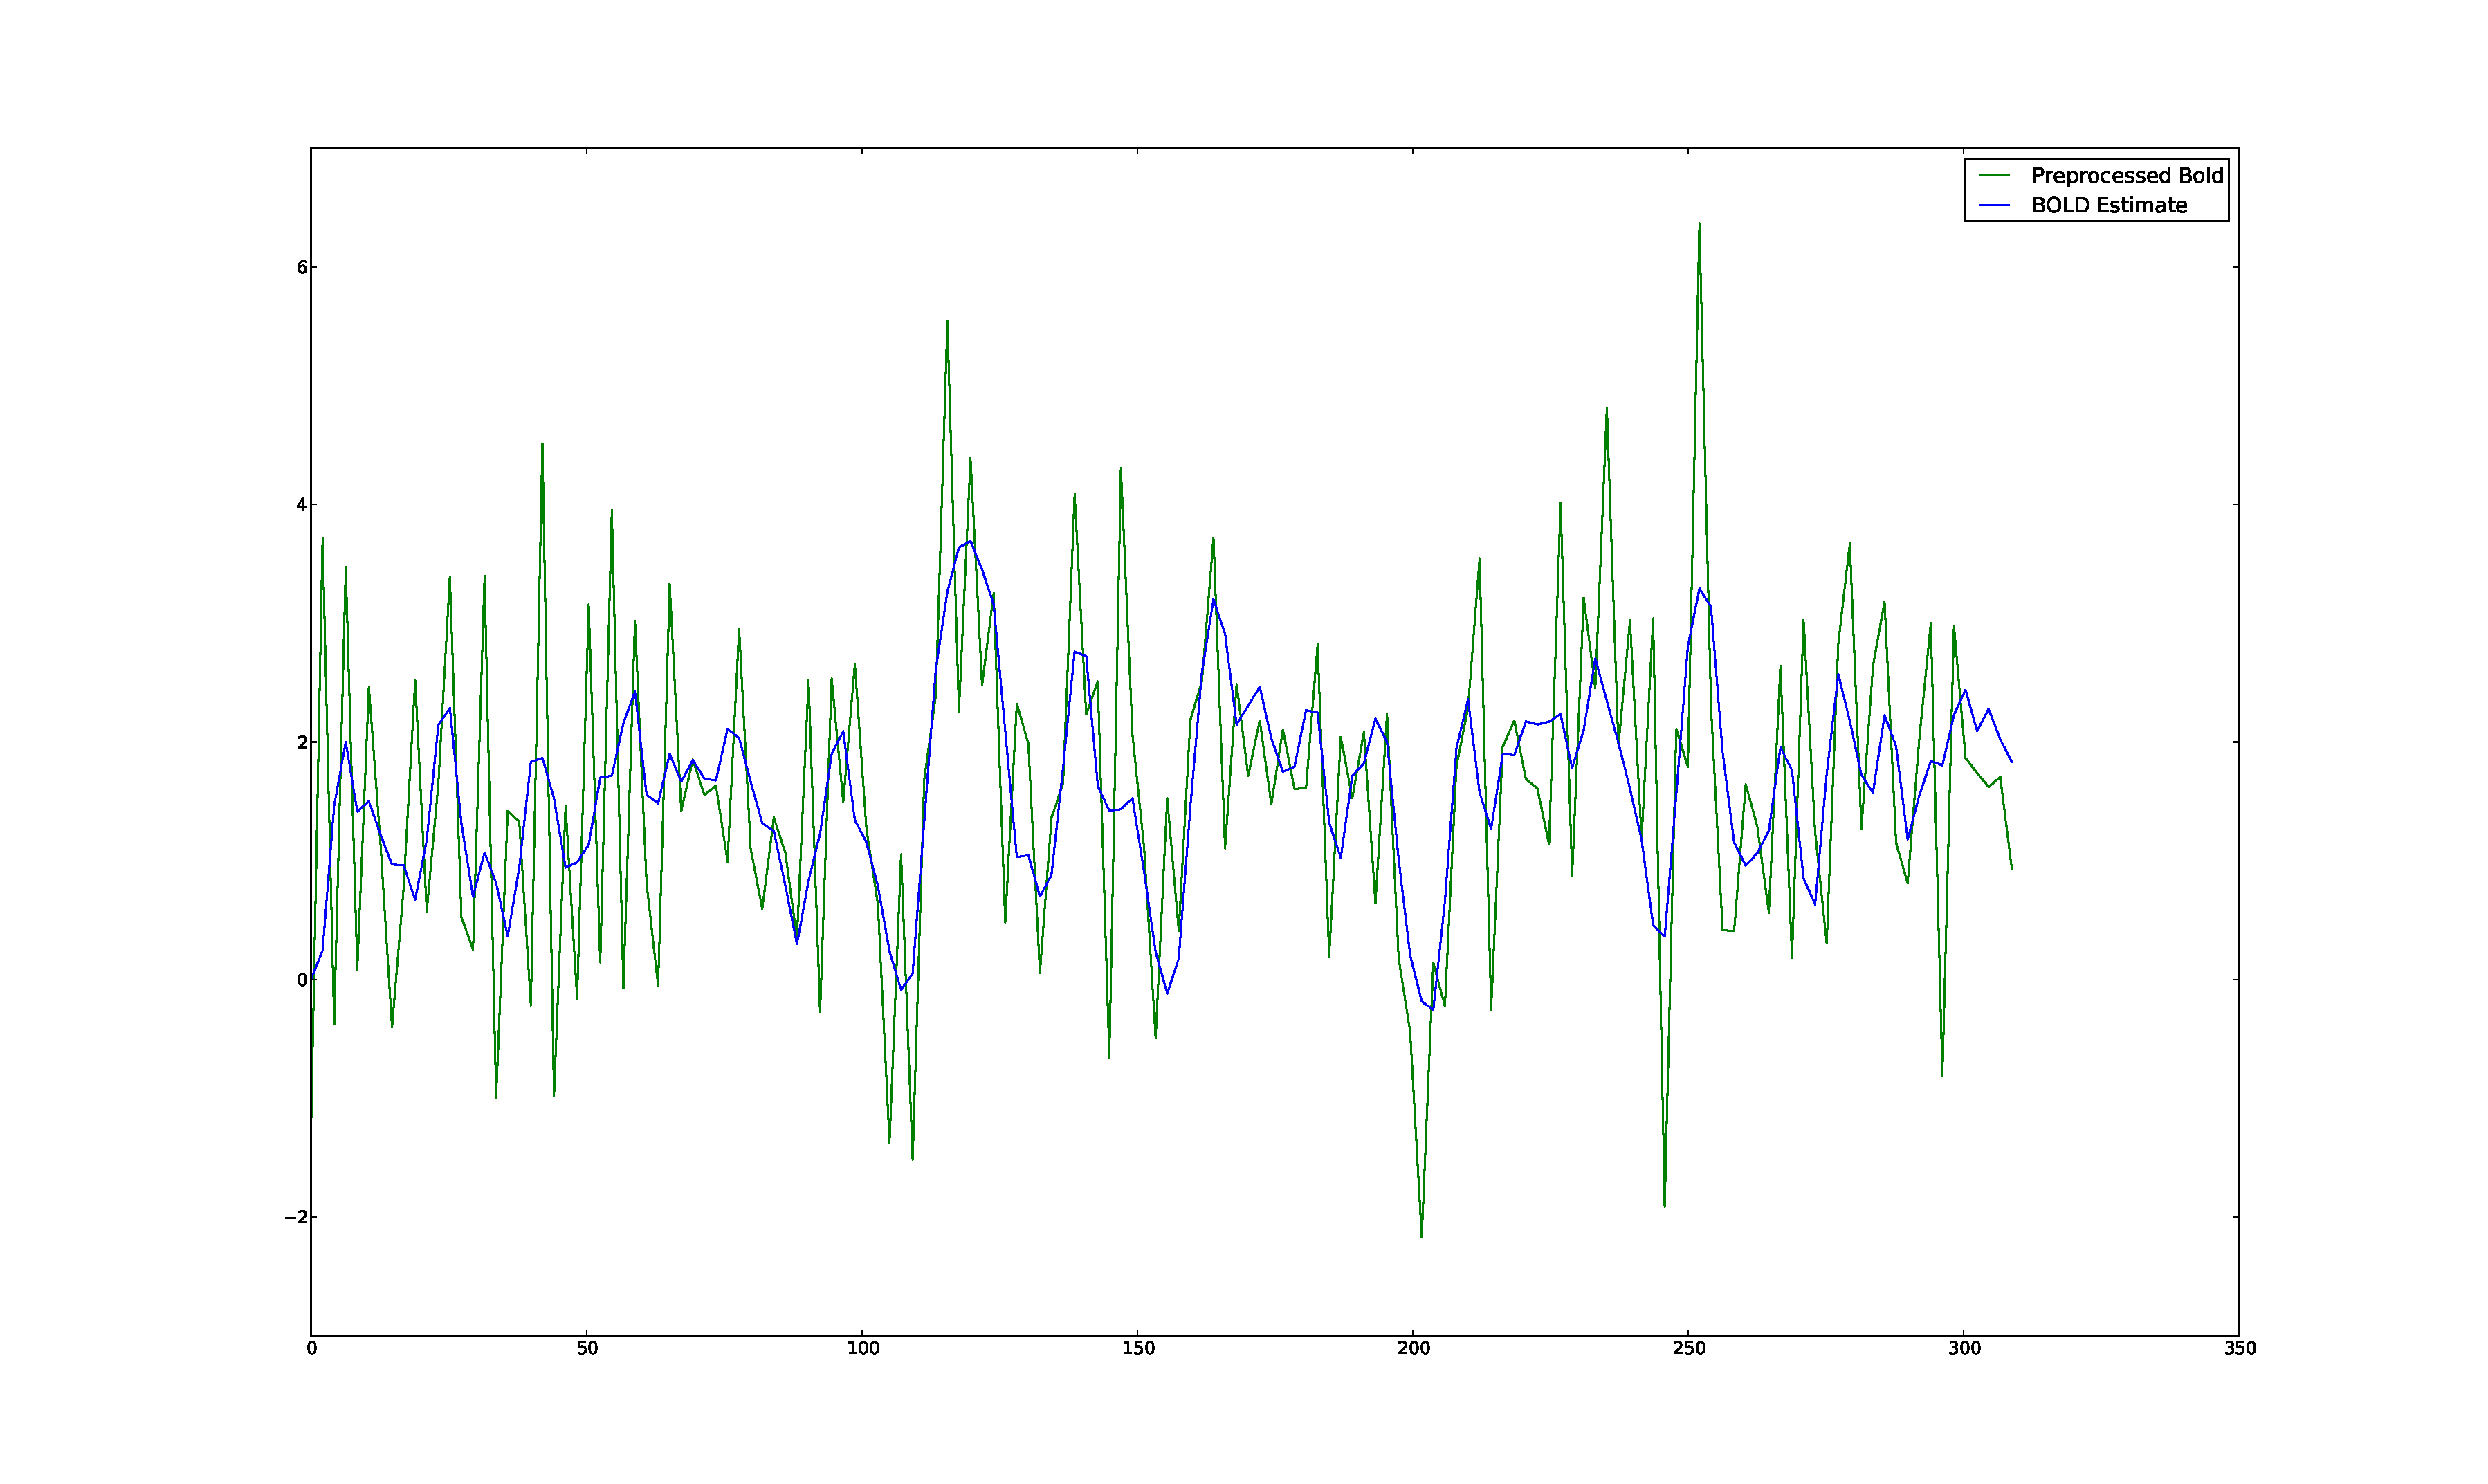
\includegraphics[clip=true,trim=5cm 1cm 4cm 1cm,width=15cm]{images/2_spm_34_12_7}}
\caption{}
\label{fig:comp2}
\end{figure}

\begin{figure}
\subfigure[Particle Filter]{\label{fig:comp3pfilter} 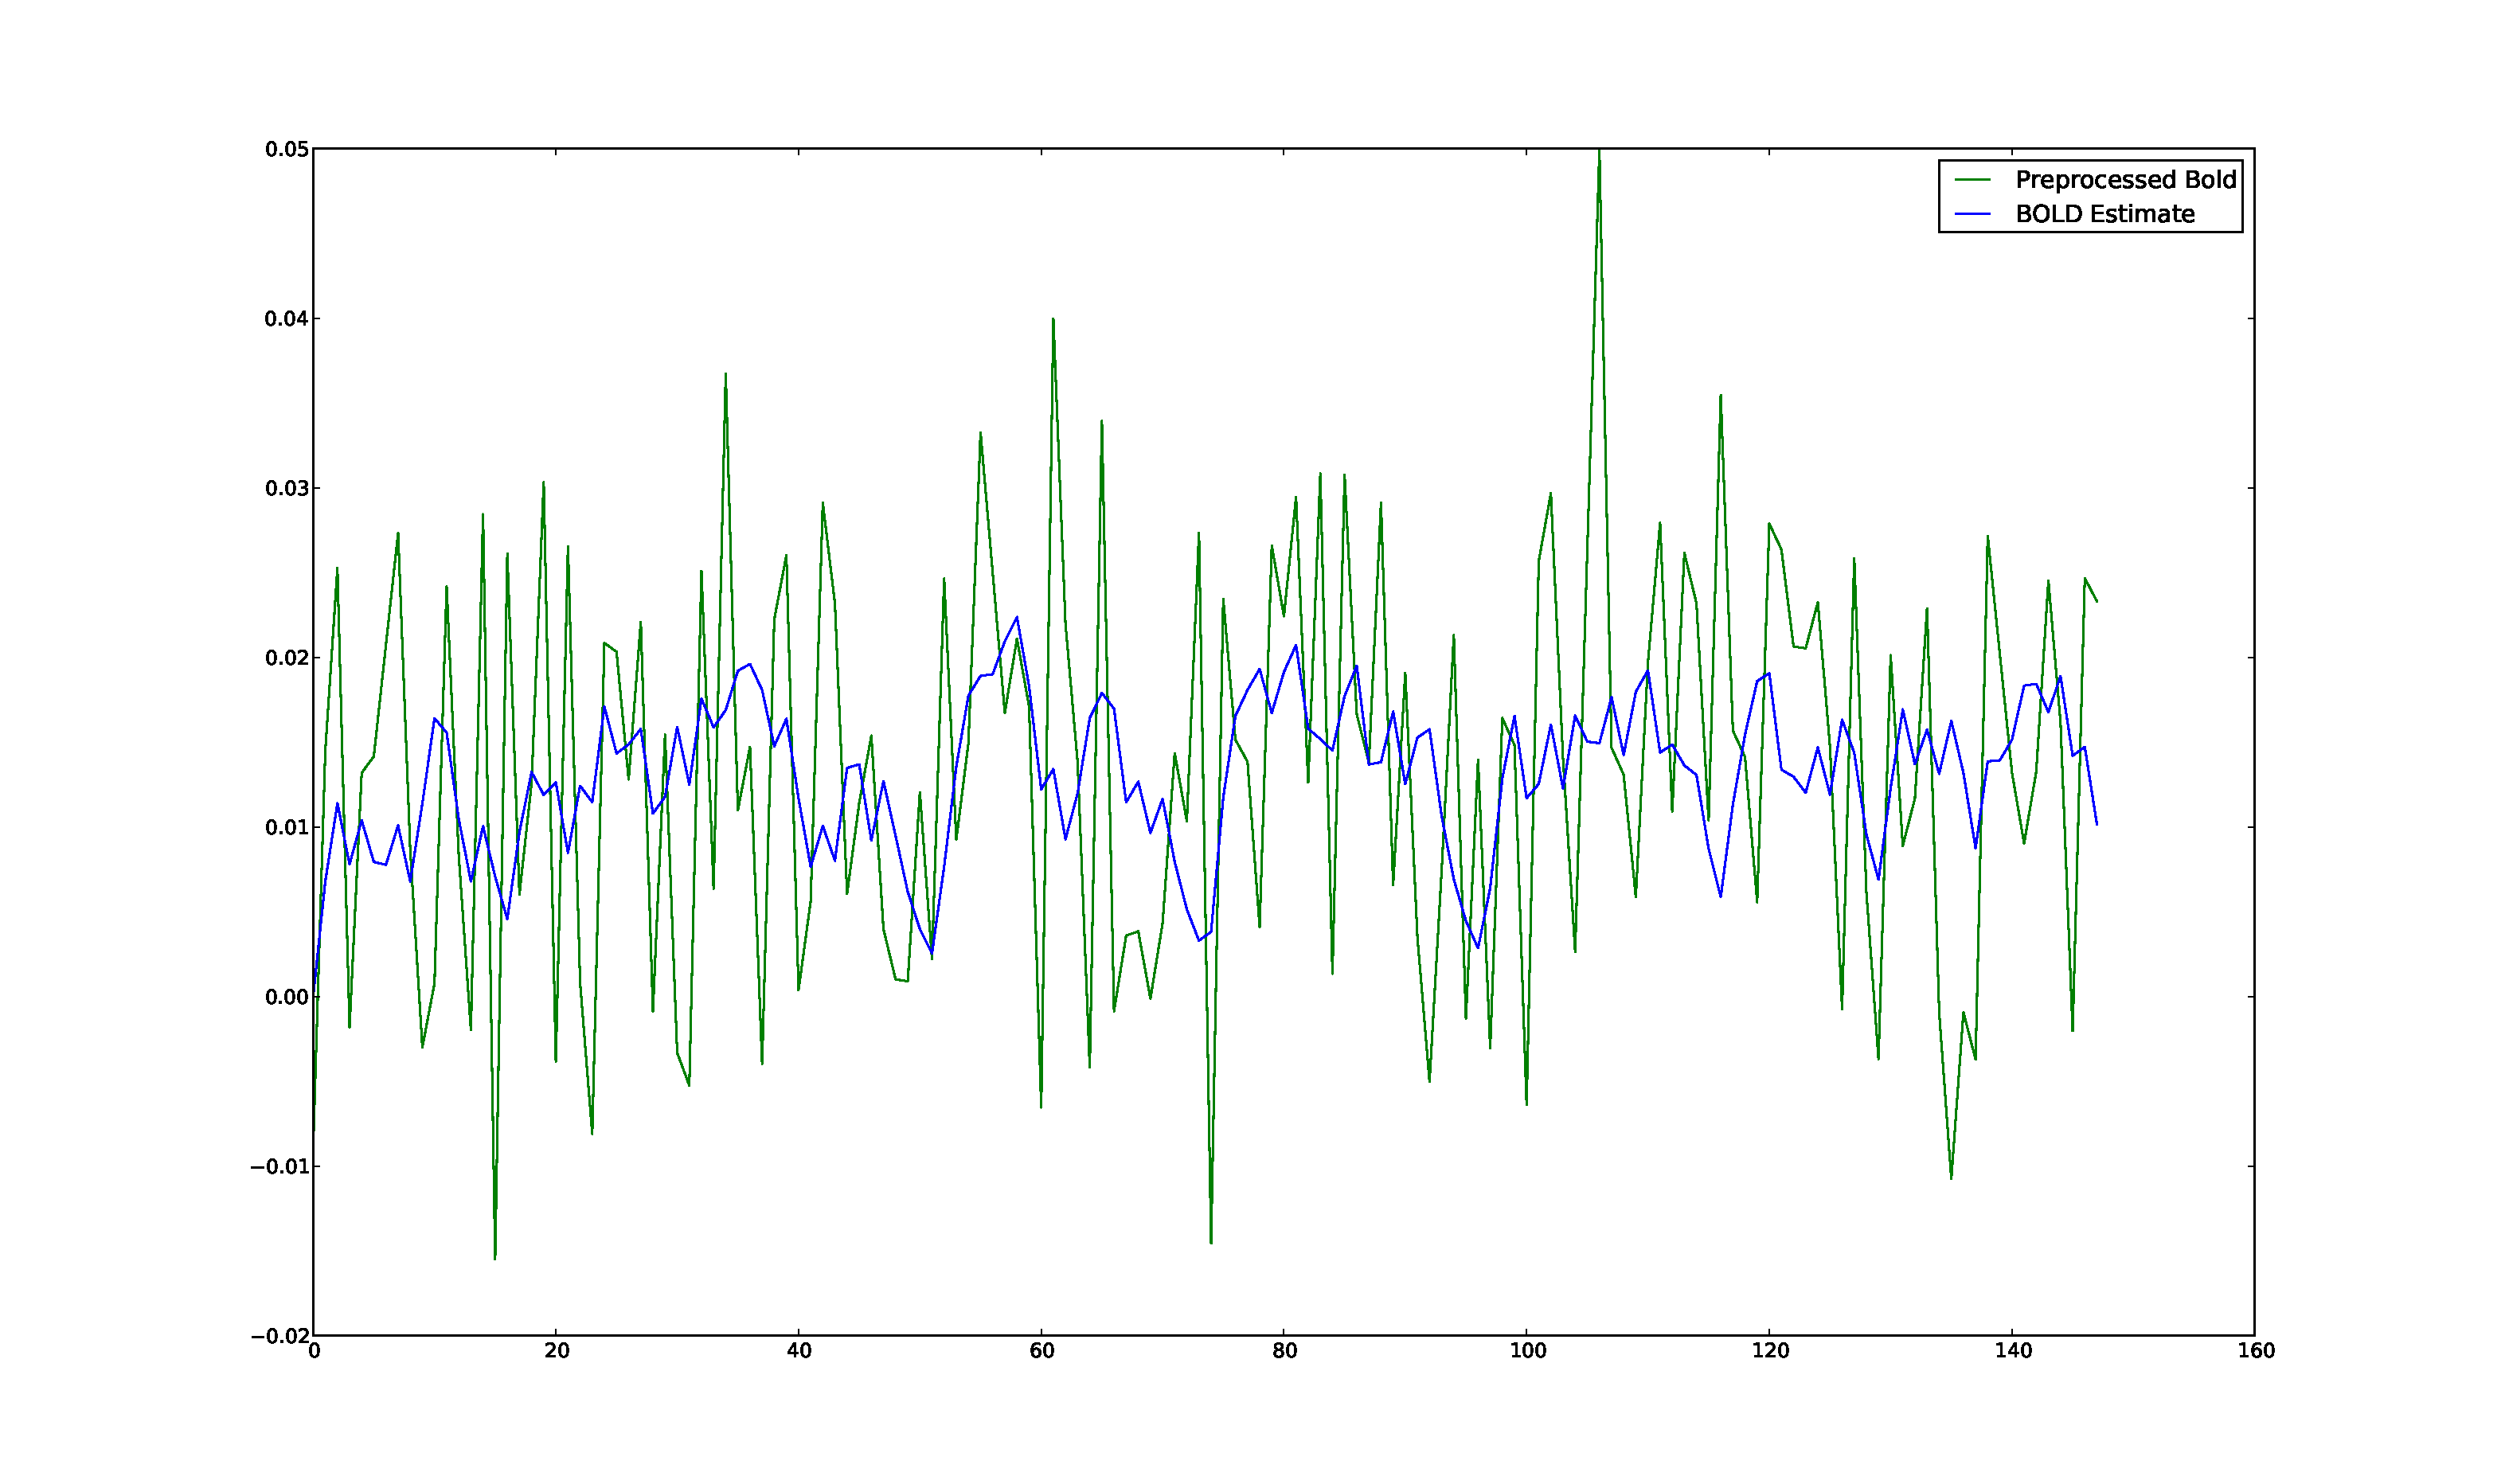
\includegraphics[clip=true,trim=5cm 1cm 4cm 1cm,width=15cm]{images/3_pfilter_23_21_7}}\\
\subfigure[SPM]{\label{fig:comp3spm} 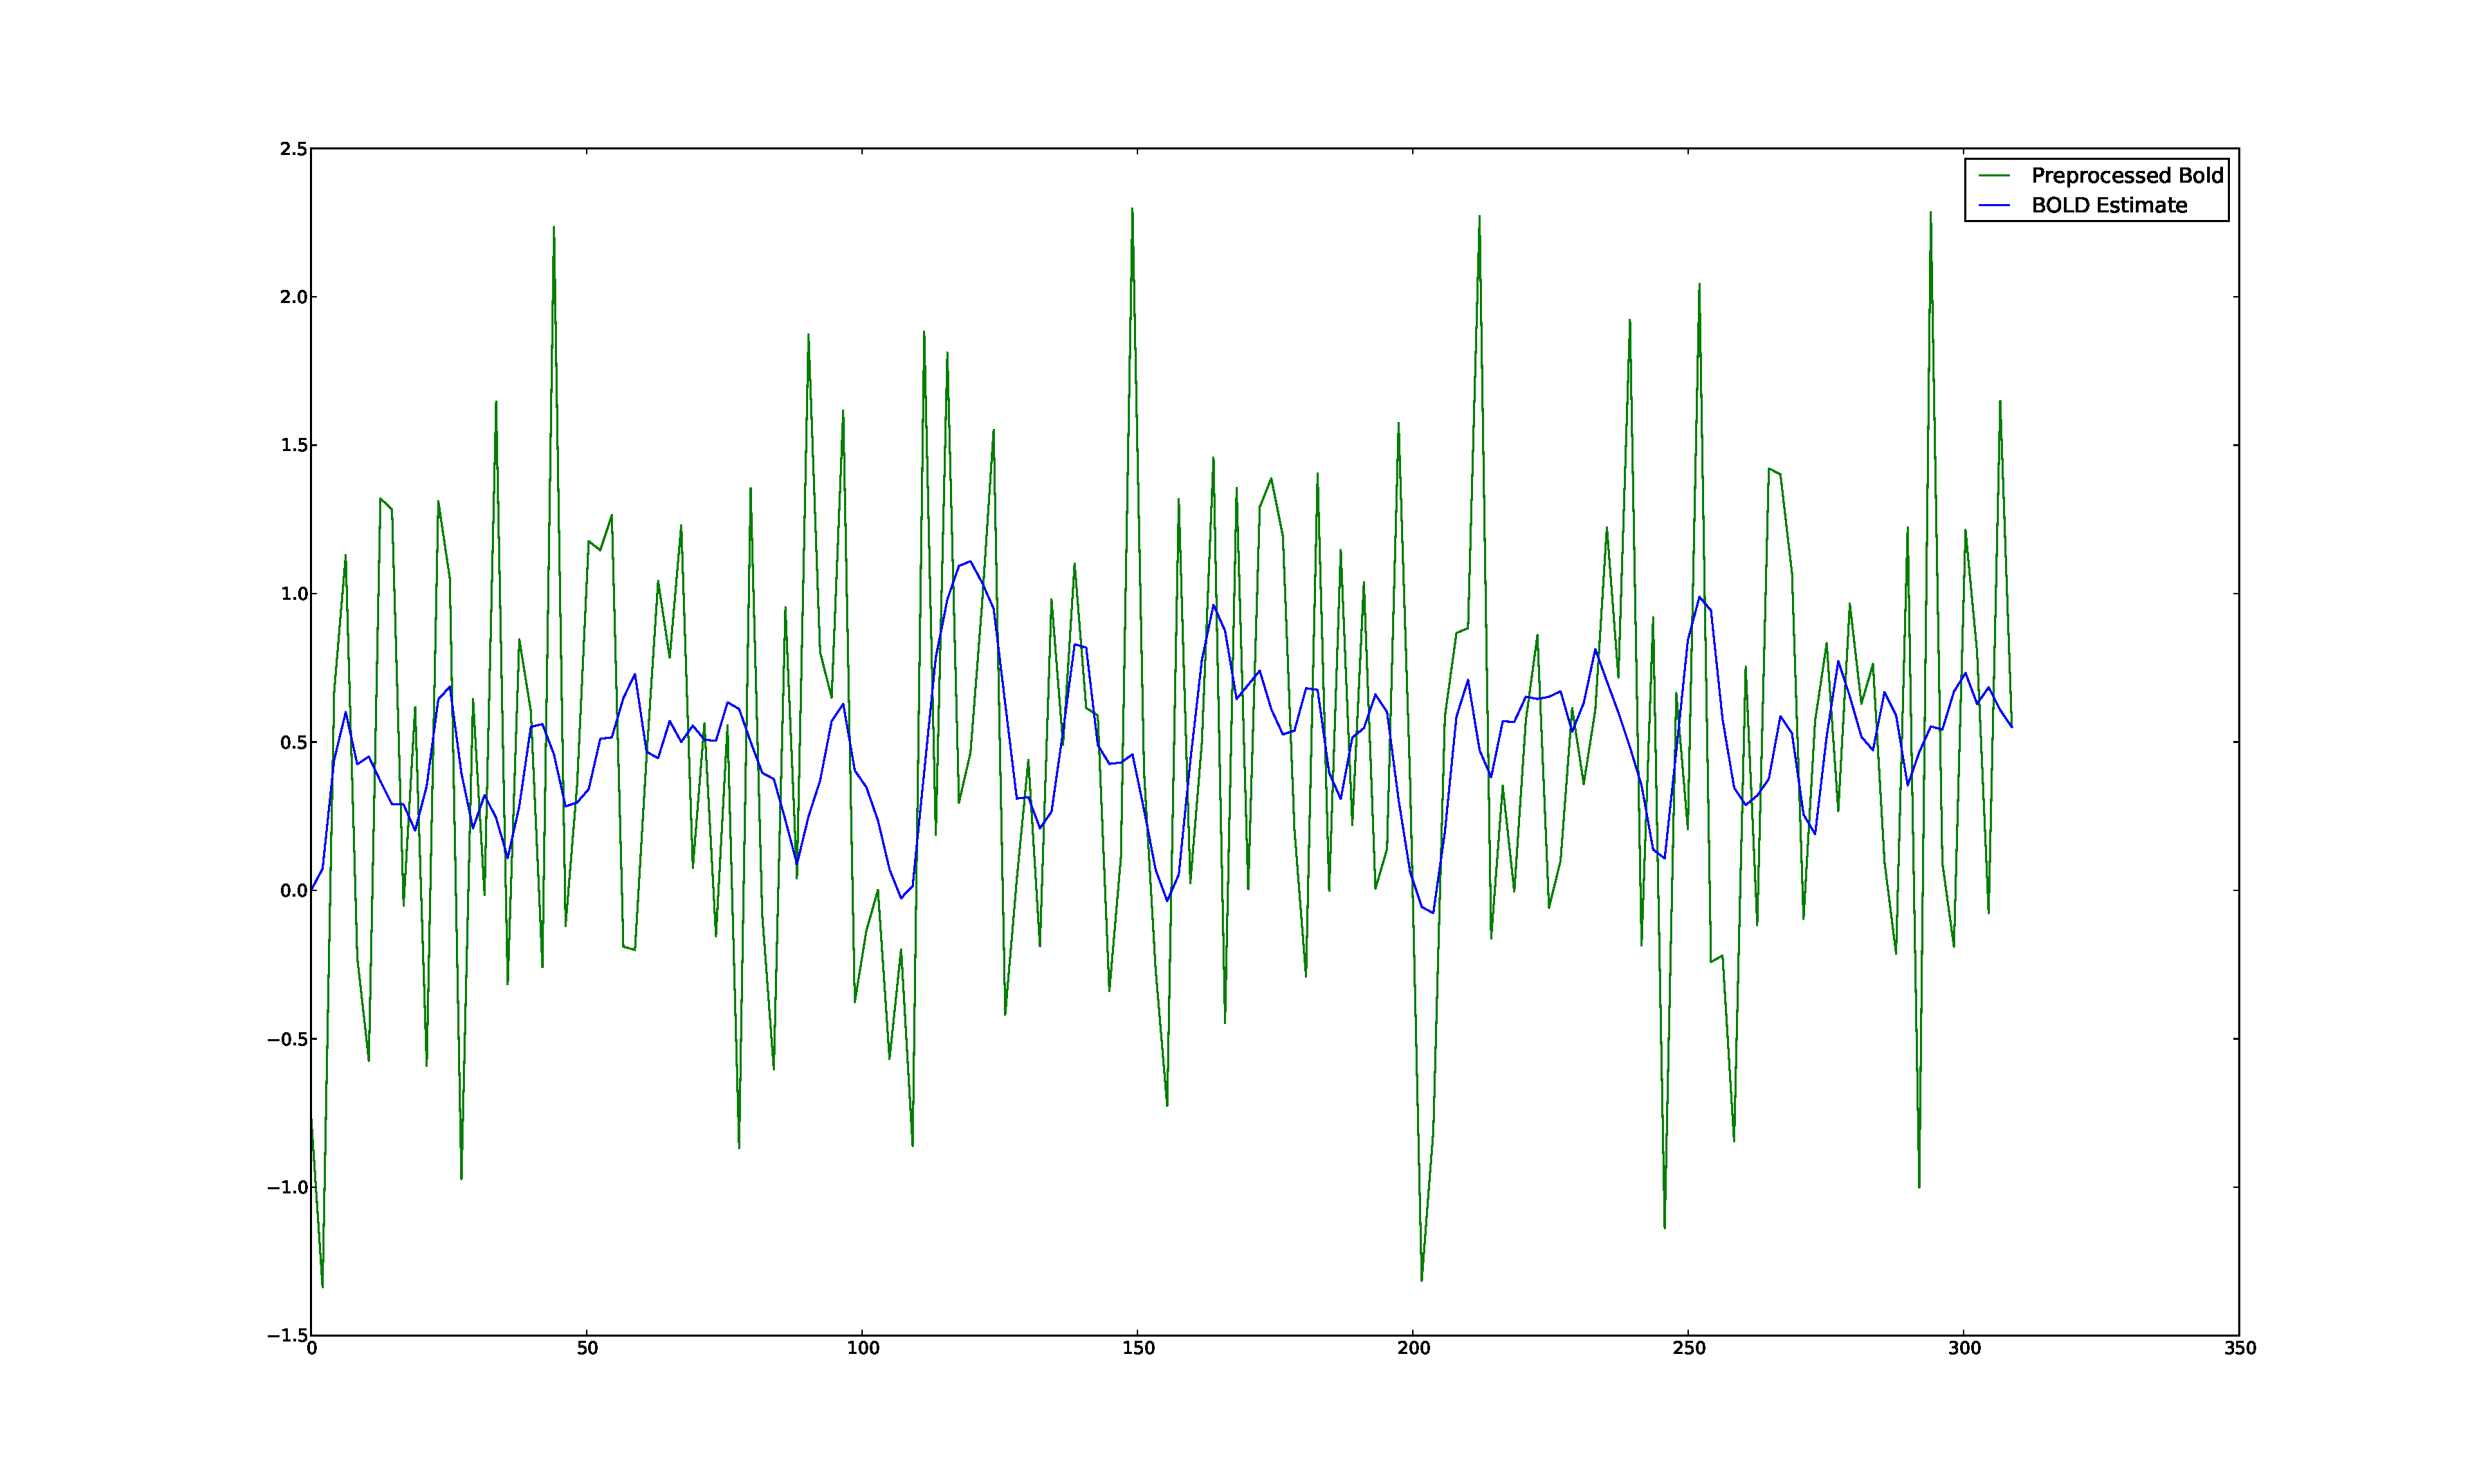
\includegraphics[clip=true,trim=5cm 1cm 4cm 1cm,width=15cm]{images/3_spm_23_21_7}}
\caption{}
\label{fig:comp3}
\end{figure}

\begin{figure}
\subfigure[Particle Filter]{\label{fig:comp4pfilter} 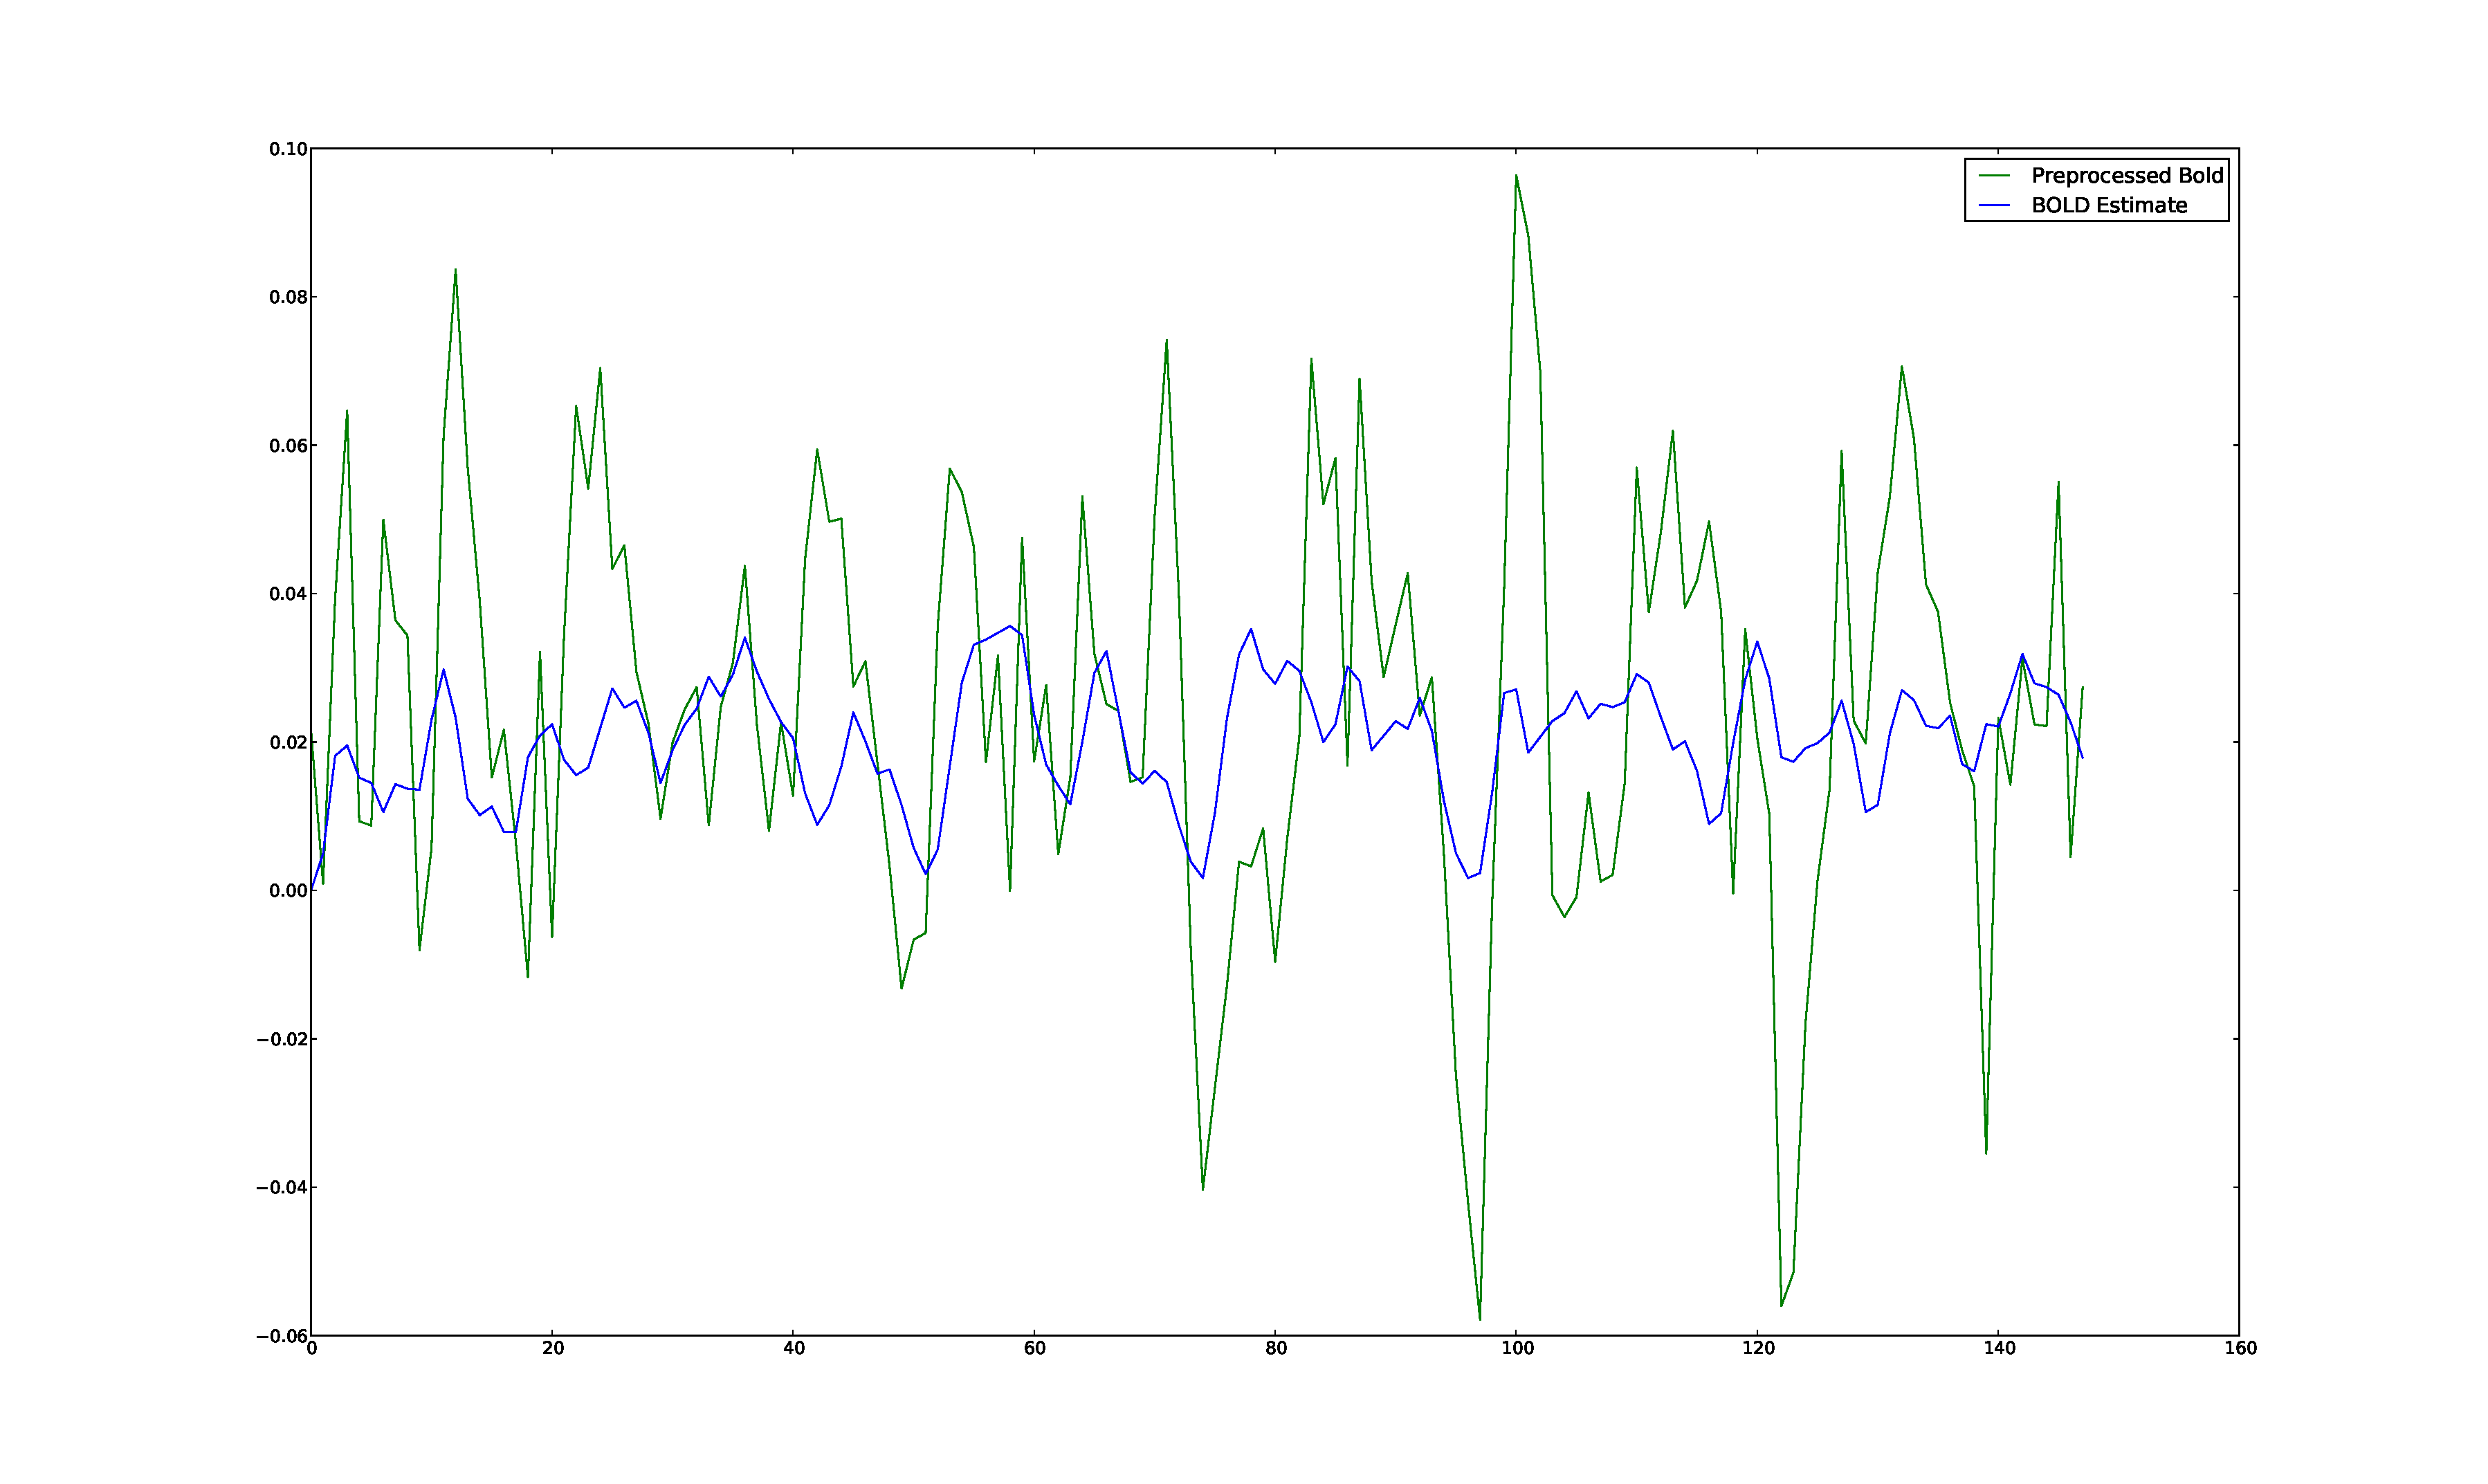
\includegraphics[clip=true,trim=5cm 1cm 4cm 1cm,width=15cm]{images/4_pfilter_26_15_7}}\\
\subfigure[SPM]{\label{fig:comp4spm} 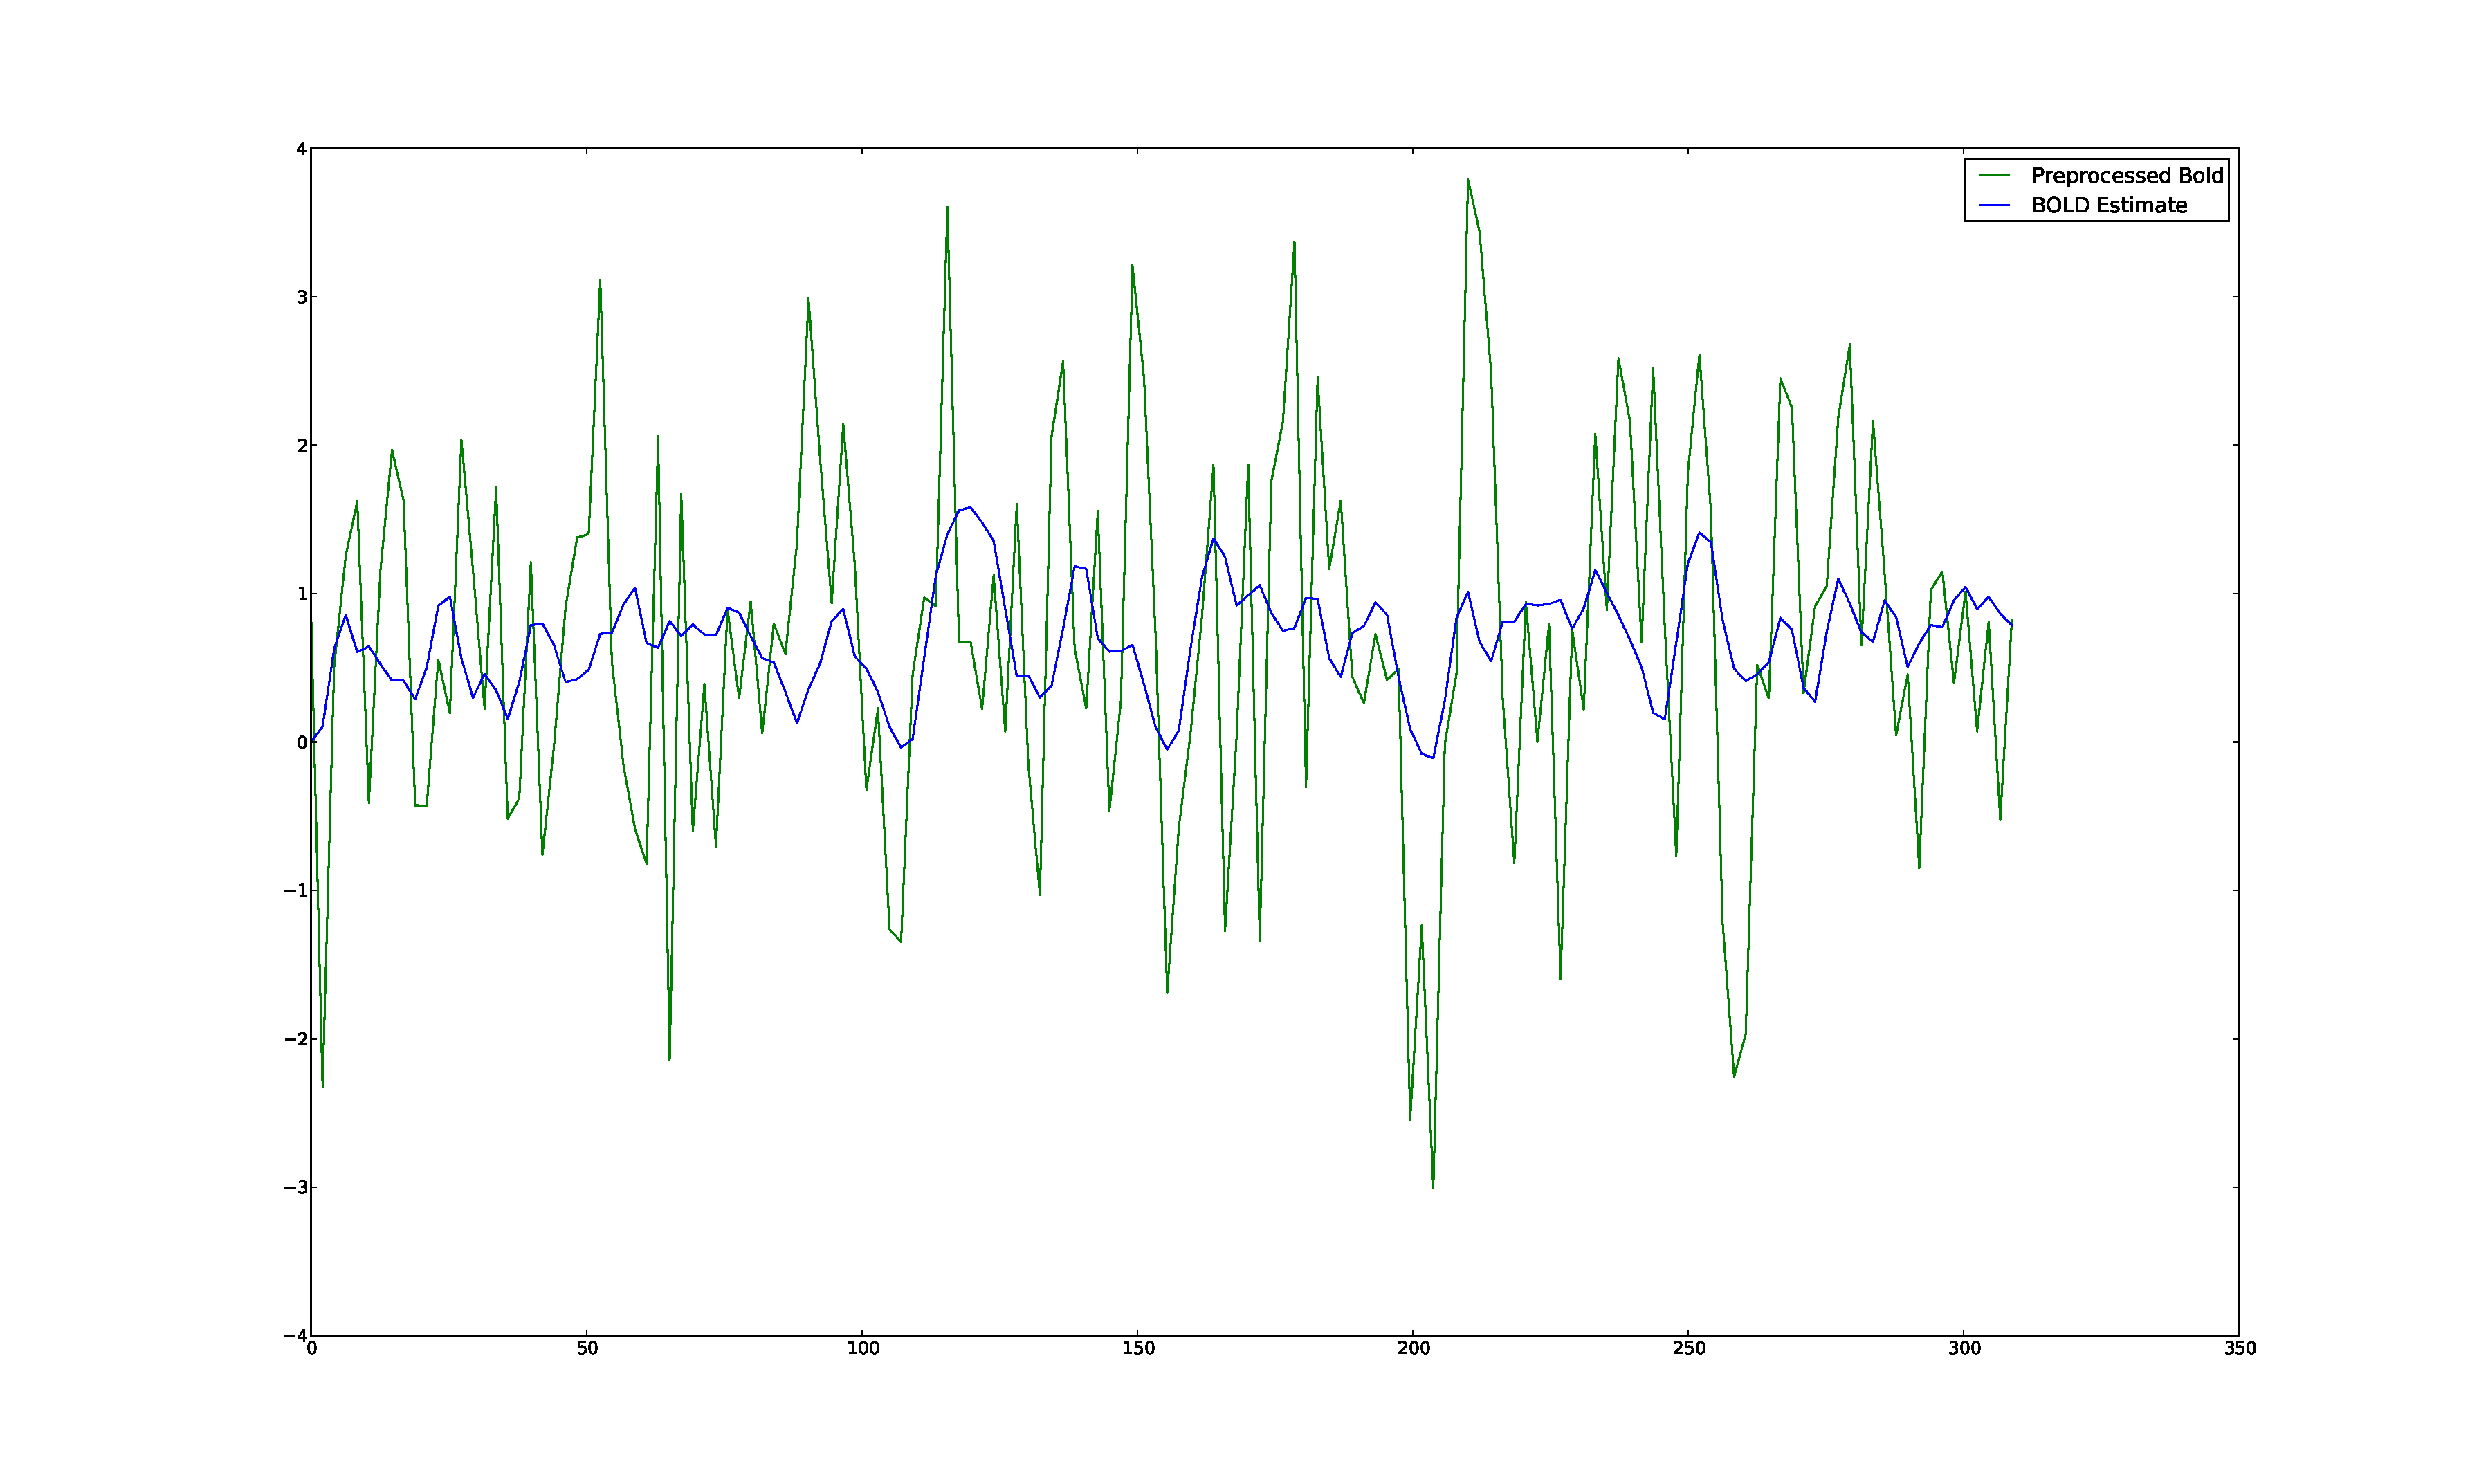
\includegraphics[clip=true,trim=5cm 1cm 4cm 1cm,width=15cm]{images/4_spm_26_15_7}}
\caption{}
\label{fig:comp4}
\end{figure}

\begin{figure}
\subfigure[Particle Filter]{\label{fig:comp5pfilter} 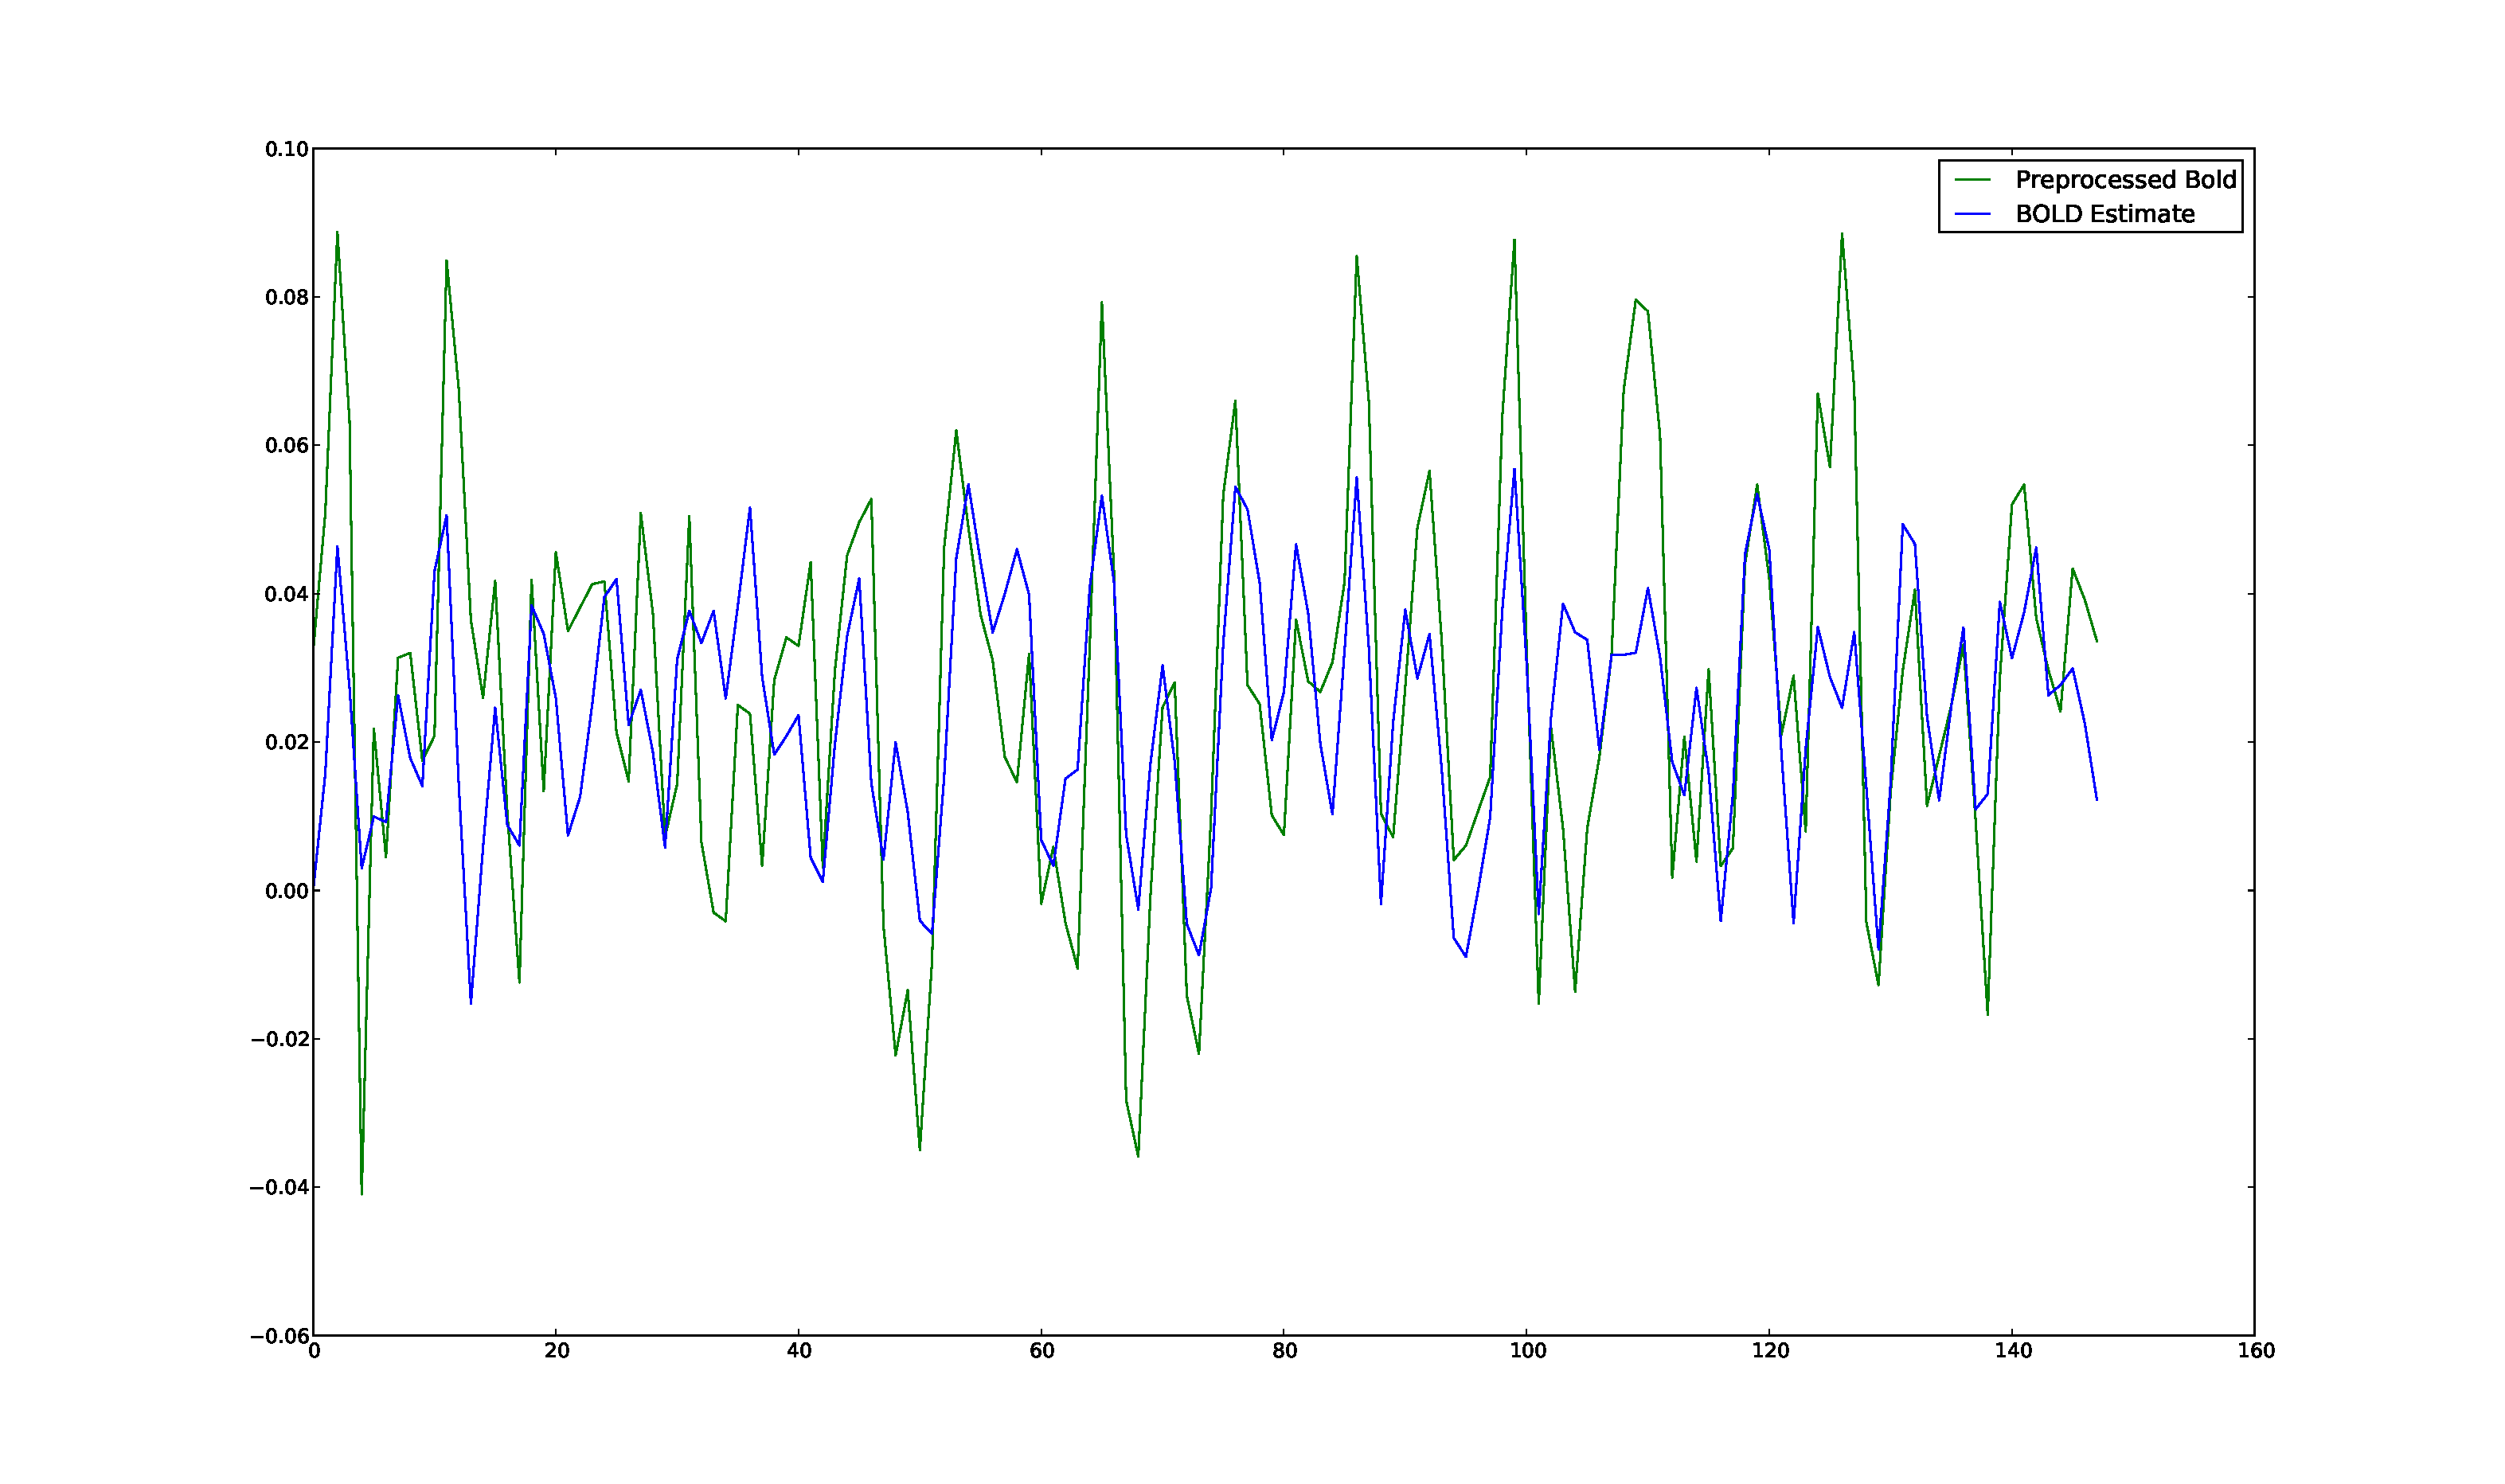
\includegraphics[clip=true,trim=5cm 1cm 4cm 1cm,width=15cm]{images/5_pfilter_25_34_25}}\\
\subfigure[SPM]{\label{fig:comp5spm} 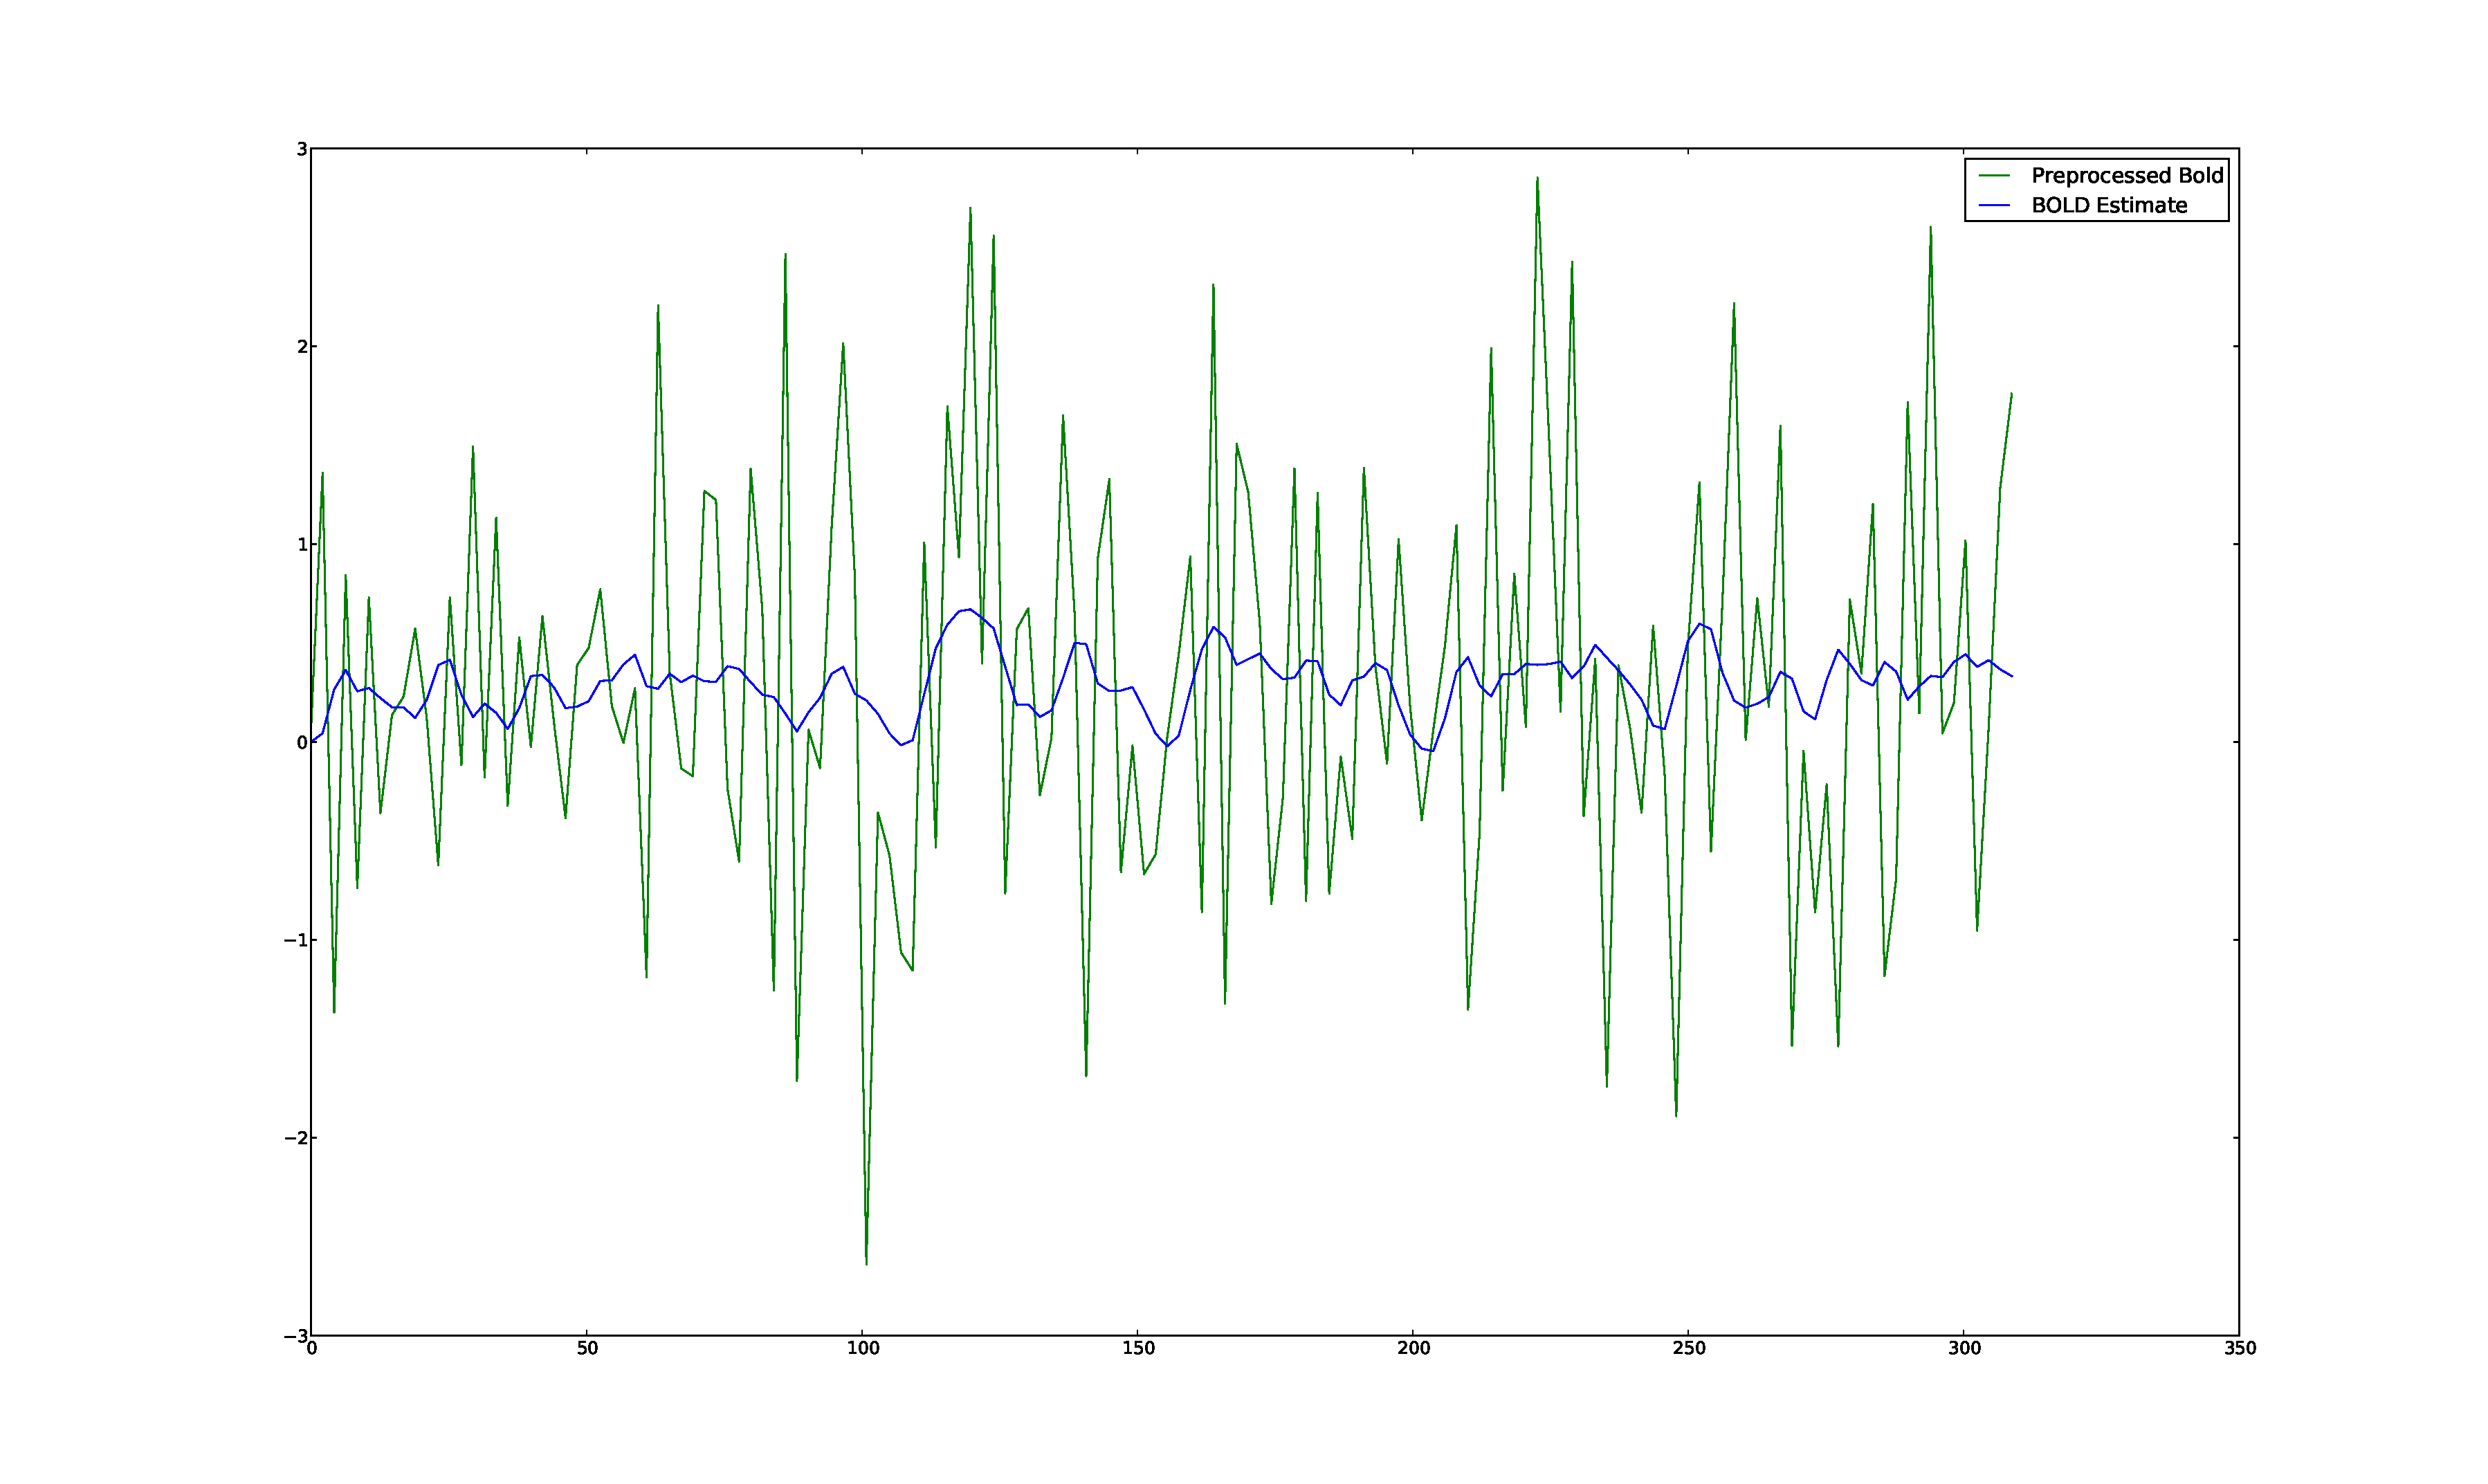
\includegraphics[clip=true,trim=5cm 1cm 4cm 1cm,width=15cm]{images/5_spm_25_34_25}}
\caption{}
\label{fig:comp5}
\end{figure}

image comparing epsilon-map with GLM activation map

